%%%%%%%% ICML 2019 EXAMPLE LATEX SUBMISSION FILE %%%%%%%%%%%%%%%%%

\documentclass{article}

% Recommended, but optional, packages for figures and better typesetting:

\usepackage{caption}
\usepackage{amsthm}
\usepackage{tabularx}
\usepackage{bm}
\usepackage{array}
\usepackage{balance}
\usepackage{amsmath}
\usepackage{amssymb}
\usepackage{multirow}
\usepackage{color}
\usepackage{microtype}
\usepackage{graphicx}
\usepackage{subfigure}
\usepackage{booktabs}
\usepackage{bbm}
\usepackage{multicol}
%\usepackage{algcompatible}


\usepackage[colorlinks,linkcolor=red,citecolor=blue]{hyperref}       % hyperlinks
\usepackage{natbib}
\allowdisplaybreaks

\DeclareMathOperator*{\Argmax}{Argmax}
\DeclareMathOperator*{\Argmin}{Argmin}

\newcommand{\var}{{\rm var}}
\newcommand{\Tr}{^{\rm T}}
\newcommand{\vtrans}[2]{{#1}^{(#2)}}
\newcommand{\kron}{\otimes}
\newcommand{\schur}[2]{({#1} | {#2})}
\newcommand{\schurdet}[2]{\left| ({#1} | {#2}) \right|}
\newcommand{\had}{\circ}
\newcommand{\diag}{{\rm diag}}
\newcommand{\invdiag}{\diag^{-1}}
\newcommand{\rank}{{\rm rank}}
\newcommand{\expt}[1]{\langle #1 \rangle}
% careful: ``null'' is already a latex command
\newcommand{\nullsp}{{\rm null}}
\newcommand{\tr}{{\rm tr}}
\renewcommand{\vec}{{\rm vec}}
\newcommand{\vech}{{\rm vech}}
\renewcommand{\det}[1]{\left| #1 \right|}
\newcommand{\pdet}[1]{\left| #1 \right|_{+}}
\newcommand{\pinv}[1]{#1^{+}}
\newcommand{\erf}{{\rm erf}}
\newcommand{\hypergeom}[2]{{}_{#1}F_{#2}}
\newcommand{\mcal}[1]{\mathcal{#1}}
\newcommand{\Rcal}{{\mathcal{R}}}
\newcommand{\Acal}{{\mathcal{A}}}
\newcommand{\Ccal}{{\mathcal{C}}}
\newcommand{\Fcal}{{\mathcal{F}}}
% boldface characters
\renewcommand{\a}{{\bf a}}
\renewcommand{\b}{{\bf b}}
\renewcommand{\c}{{\bf c}}
\renewcommand{\d}{{\rm d}}  % for derivatives
\newcommand{\e}{{\bf e}}
\newcommand{\f}{{\bf f}}
\newcommand{\g}{{\bf g}}
\newcommand{\h}{{\bf h}}
\newcommand{\bi}{{\bf i}}
\newcommand{\bj}{{\bf j}}
\newcommand{\bK}{{\bf K}}
\newcommand{\Kcal}{{\mathcal{K}}}
% in Latex2e this must be renewcommand
\renewcommand{\k}{{\bf k}}
\newcommand{\m}{{\bf m}}
\newcommand{\mhat}{{\overline{m}}}
\newcommand{\tm}{{\tilde{m}}}
\newcommand{\n}{{\bf n}}
\renewcommand{\o}{{\bf o}}
\newcommand{\p}{{\bf p}}
\newcommand{\q}{{\bf q}}
\renewcommand{\r}{{\bf r}}
\newcommand{\s}{{\bf s}}
\renewcommand{\t}{{\bf t}}
\renewcommand{\u}{{\bf u}}
\renewcommand{\v}{{\bf v}}
\newcommand{\w}{{\bf w}}
\newcommand{\x}{{\bf x}}
\newcommand{\y}{{\bf y}}
\newcommand{\z}{{\bf z}}
\newcommand{\bl}{{\bf l}}
\newcommand{\A}{{\bf A}}
\newcommand{\B}{{\bf B}}
\newcommand{\C}{{\bf C}}
\newcommand{\D}{{\bf D}}
\newcommand{\Dcal}{\mathcal{D}}
\newcommand{\E}{{\bf E}}
\newcommand{\F}{{\bf F}}
\newcommand{\G}{{\bf G}}
\newcommand{\Gcal}{{\mathcal{G}}}
\renewcommand{\H}{{\bf H}}
\newcommand{\I}{{\bf I}}
\newcommand{\J}{{\bf J}}
\newcommand{\K}{{\bf K}}
\renewcommand{\L}{{\bf L}}
%\newcommand{\Lcal}{{\mathcal{L}}}
\newcommand{\M}{{\bf M}}
\newcommand{\Mcal}{{\mathcal{M}}}
\newcommand{\N}{\mathcal{N}}  % for normal density
%\newcommand{\N}{{\bf N}}
\newcommand{\bupeta}{\boldsymbol{\upeta}}
\renewcommand{\O}{{\bf O}}
\renewcommand{\P}{{\bf P}}
\newcommand{\Q}{{\bf Q}}
\newcommand{\R}{{\bf R}}
\renewcommand{\S}{{\bf S}}
\newcommand{\Scal}{{\mathcal{S}}}
\newcommand{\T}{{\bf T}}
\newcommand{\Tcal}{{\mathcal{T}}}
\newcommand{\U}{{\bf U}}
\newcommand{\Ucal}{{\mathcal{U}}}
\newcommand{\tU}{{\tilde{\U}}}
\newcommand{\tUcal}{{\tilde{\Ucal}}}
\newcommand{\V}{{\bf V}}
\newcommand{\W}{{\bf W}}

\newcommand{\Ocal}[1]{{\mathcal{O}\left( #1  \right)}}
\newcommand{\Omegacal}[1]{{\Omega \left( #1 \right)}}
\newcommand{\Pcal}{{\mathcal{P}}}
\newcommand{\Hcal}{{\mathcal{H}}}
\newcommand{\Wcal}{{\mathcal{W}}}
\newcommand{\X}{{\bf X}}
\newcommand{\Xcal}{{\mathcal{X}}}
\newcommand{\Y}{{\bf Y}}
\newcommand{\Ycal}{{\mathcal{Y}}}
\newcommand{\Z}{{\bf Z}}
\newcommand{\Zcal}{{\mathcal{Z}}}

% this is for latex 2.09
% unfortunately, the result is slanted - use Latex2e instead
%\newcommand{\bfLambda}{\mbox{\boldmath$\Lambda$}}
% this is for Latex2e
\newcommand{\bfLambda}{\boldsymbol{\Lambda}}

% Yuan Qi's boldsymbol
\newcommand{\bsigma}{\boldsymbol{\sigma}}
\newcommand{\balpha}{\boldsymbol{\alpha}}
\newcommand{\bpsi}{\boldsymbol{\psi}}
\newcommand{\bphi}{\boldsymbol{\phi}}
\newcommand{\bbeta}{\boldsymbol{\beta}}
\newcommand{\bepsi}{\boldsymbol{\epsilon}}
\newcommand{\Beta}{\boldsymbol{\eta}}
\newcommand{\btau}{\boldsymbol{\tau}}
\newcommand{\bvarphi}{\boldsymbol{\varphi}}
\newcommand{\bzeta}{\boldsymbol{\zeta}}

\newcommand{\blambda}{\boldsymbol{\lambda}}
\newcommand{\bLambda}{\mathbf{\Lambda}}

\newcommand{\btheta}{\boldsymbol{\theta}}
\newcommand{\bTheta}{\boldsymbol{\Theta}}
\newcommand{\bpi}{\boldsymbol{\pi}}
\newcommand{\bxi}{\boldsymbol{\xi}}
\newcommand{\bSigma}{\boldsymbol{\Sigma}}
\newcommand{\bPi}{\boldsymbol{\Pi}}
\newcommand{\bOmega}{\boldsymbol{\Omega}}
%\newcommand{\bLambda}{\boldsymbol{\Lambda}}

\newcommand{\hatu}{\hat{\bf u}}



\newcommand{\bgamma}{\boldsymbol{\gamma}}
\newcommand{\bGamma}{\boldsymbol{\Gamma}}
\newcommand{\bUpsilon}{\boldsymbol{\Upsilon}}



\newcommand{\bmu}{\boldsymbol{\mu}}
\newcommand{\1}{{\bf 1}}
\newcommand{\0}{{\bf 0}}


\newcommand{\proj}[1]{{\rm proj}\negmedspace\left[#1\right]}
\newcommand{\argmin}{\operatornamewithlimits{argmin}}
\newcommand{\argmax}{\operatornamewithlimits{argmax}}

\newcommand{\dif}{\mathrm{d}}
\newcommand{\lrincir}[1]{\left( #1 \right)}
\newcommand{\abs}[1]{\lvert#1\rvert}
\newcommand{\norm}[1]{\lVert#1\rVert}
\newcommand{\lrnorm}[1]{\left\lVert#1\right\rVert}
\newcommand{\lrangle}[1]{\left\langle#1 \right\rangle}

\newcommand{\ie}{{{i.e.,}}\xspace}
\newcommand{\eg}{{{\em e.g.,}}\xspace}
\newcommand{\EE}{\mathop{\mathbb{E}}}
\newcommand{\RR}{\mathbb{R}}
\newcommand{\sbr}[1]{\left[#1\right]}
\newcommand{\rbr}[1]{\left(#1\right)}
\newcommand{\Lcal}[1]{\mathcal{L}^{#1}_{D_1,D_2}}


\newcommand{\refabove}[2]{\displaystyle_{#1}^{(#2)}}
\newcommand{\refabovecir}[2]{\displaystyle_{#1}^{#2}}



 \newtheorem{Definition}{\bf{Definition}}
 \newtheorem{Theorem}{\bf{Theorem}}
 \newtheorem{reTheorem}[Theorem]{\bf{Theorem}}
 \newtheorem{Lemma}{\bf{Lemma}}
 \newtheorem{reLemma}[Lemma]{\bf{Lemma}}
 \newtheorem{Corollary}{\bf{Corollary}}
 \newtheorem{reCorollary}[Corollary]{\bf{Corollary}}
 \newtheorem{Assumption}{\bf{Assumption}}
 \newtheorem{Proposition}{\bf{Proposition}}
 \newtheorem{Remark}{\bf{Remark}}



 % for professional tables

% hyperref makes hyperlinks in the resulting PDF.
% If your build breaks (sometimes temporarily if a hyperlink spans a page)
% please comment out the following usepackage line and replace
% \usepackage{icml2019} with \usepackage[nohyperref]{icml2019} above.
\usepackage{hyperref}

% Attempt to make hyperref and algorithmic work together better:
\newcommand{\theHalgorithm}{\arabic{algorithm}}

% Use the following line for the initial blind version submitted for review:
\usepackage{icml2019}

% If accepted, instead use the following line for the camera-ready submission:
%\usepackage[accepted]{icml2019}

% The \icmltitle you define below is probably too long as a header.
% Therefore, a short form for the running title is supplied here:
\icmltitlerunning{Decentralized Online Learning: Exchanging Local Models to Track Dynamics}




\hypersetup{draft}% need to be commit before submitting paper
\begin{document}

\twocolumn[
\icmltitle{Decentralized Online Learning: Exchanging Local Models to Track Dynamics}

% It is OKAY to include author information, even for blind
% submissions: the style file will automatically remove it for you
% unless you've provided the [accepted] option to the icml2019
% package.

% List of affiliations: The first argument should be a (short)
% identifier you will use later to specify author affiliations
% Academic affiliations should list Department, University, City, Region, Country
% Industry affiliations should list Company, City, Region, Country

% You can specify symbols, otherwise they are numbered in order.
% Ideally, you should not use this facility. Affiliations will be numbered
% in order of appearance and this is the preferred way.
\icmlsetsymbol{equal}{*}

\begin{icmlauthorlist}
\icmlauthor{Aeiau Zzzz}{equal,to}
\icmlauthor{Bauiu C.~Yyyy}{equal,to,goo}
\icmlauthor{Cieua Vvvvv}{goo}
\icmlauthor{Iaesut Saoeu}{ed}
\icmlauthor{Fiuea Rrrr}{to}
\icmlauthor{Tateu H.~Yasehe}{ed,to,goo}
\icmlauthor{Aaoeu Iasoh}{goo}
\icmlauthor{Buiui Eueu}{ed}
\icmlauthor{Aeuia Zzzz}{ed}
\icmlauthor{Bieea C.~Yyyy}{to,goo}
\icmlauthor{Teoau Xxxx}{ed}
\icmlauthor{Eee Pppp}{ed}
\end{icmlauthorlist}

\icmlaffiliation{to}{Department of Computation, University of Torontoland, Torontoland, Canada}
\icmlaffiliation{goo}{Googol ShallowMind, New London, Michigan, USA}
\icmlaffiliation{ed}{School of Computation, University of Edenborrow, Edenborrow, United Kingdom}

\icmlcorrespondingauthor{Cieua Vvvvv}{c.vvvvv@googol.com}
\icmlcorrespondingauthor{Eee Pppp}{ep@eden.co.uk}

% You may provide any keywords that you
% find helpful for describing your paper; these are used to populate
% the "keywords" metadata in the PDF but will not be shown in the document
\icmlkeywords{Machine Learning, ICML}

\vskip 0.3in
]

% this must go after the closing bracket ] following \twocolumn[ ...

% This command actually creates the footnote in the first column
% listing the affiliations and the copyright notice.
% The command takes one argument, which is text to display at the start of the footnote.
% The \icmlEqualContribution command is standard text for equal contribution.
% Remove it (just {}) if you do not need this facility.

%\printAffiliationsAndNotice{}  % leave blank if no need to mention equal contribution
\printAffiliationsAndNotice{\icmlEqualContribution} % otherwise use the standard text.


\begin{abstract}
In this paper, we consider online learning in the decentralized setting, which is motivated by the application scenario where users want to take benefits from the data from other users, but do not want to share their private data to a third party or other users. Instead, they can only share their private prediction model, e.g., recommendation model. We study the decentralized online gradient method in which each user maintains a private model and share its private model with its neighbors (or users he/she trusts) periodically. In addition, to consider more practical scenario we allow users' interest changing over time (it means that the optimal model changes over time), unlike most online works which assume that the optimal prediction model is constant. We show that decentralized online gradient (DOG) can efficiently and effectively propagate the values in all private data without sharing them to track the dynamics of users' interest, by proving a tight dynamic regret $\Ocal{n\sqrt{TM} + \sqrt{nTM}\sigma}$ for DOG where $n$ is the number of users, $T$ is the number of time steps, $M$ measures the dynamics (this is, how much the users' interest changes over time), and $\sigma$ measures the randomness of the private data. Empirical studies are also conducted to validate our analysis. This study indicates the possibility of a new framework of data service: all users can take benefit from their private data without sharing them.
\end{abstract}


\section{Introduction}
\label{sect_introduction}
\label{sect_introduction}

Online learning has been studied for decades of years in machine learning literatures~\citep{Hazan2016Introduction,ShalevShwartz:2012dz,Duchi:2011}. The goal of online learning generally is to incrementally learn predictions models to minimize the sum of all the online loss functions (cumulative loss), which is usually determined by a squence of examples that arrives sequentially. To quantify the efficacy of an online learning algorithm, the community introduced a performance measure called \textit{static regret}, which is the difference between the cumulative losses suffered by the online algorithm and that suffered by the best model which can observe all the loss functions. The best static regret of a sequential online convex optimization method is  $\Ocal{\sqrt{T}}$ and $\Ocal{\log T}$  for convex and strongly convex loss functions, respectively \citep{Hazan2016Introduction,ShalevShwartz:2012dz}.

Different with traditional online learning, online learning in decentralized networks (or Decentralized Online Learning) assumes that a network of computational nodes can communicate between neighors to solve an online learning problem, in which each computational node will receive a stream of online losses. Suppose we have $n$ workers, among which the $i$-th one will receive the $t$-th loss $f_{i,t}$ at the $t-$th iteration. Then, the goal of Decentralized Online Learning usually is to minimize its static regret, which is defined as the difference between the cumulative loss over all the nodes and steps and that of the best model which knows all the loss function beforehand. Decentralized Online Learning enjoys many advantages for real-world large-scale applications. Firstly, it avoid collecting all the loss functions to one node, which will result in heavy communication cost for the network and extremely high computational cost for one node. Secondly, it can help many data providers collaborate to better minimize their cumulative loss, while at the same time protect the data privacy as much as possible. 

The static regret assumes that the best model keeps unchanged during the entire learning process, however this does not hold in some real applications. For example, one's favorite style of musics may change over time as his/her situation. To solve this issue, the dynamic regret is introduced, which generally measure the difference between the cumulative loss suffered by the decentralized online learning algorithm and that suffered by a dynamic sequence of models. This dynamic sequence of models can not only observe all the loss functions beforehand, but also changes over time with the amount of changes less than a budget. In this paper, we mainly prove that decentralized online gradient can achieve a dynamic regret  of $\Ocal{n\sqrt{TM} + \sqrt{nTM}\sigma}$ where $n$ is the number of users, $T$ is the number of time steps, $M$ measures the dynamics budget, and $\sigma$ measures the randomness of the private data. 


\paragraph{Notations and definitions}
In the paper, we make the following notations.
\begin{itemize}
\item For any $i\in[n]$ and $t\in[T]$, the random variable $\xi_{i,t}$ is subject to a distribution $D_{i,t}$, that is, $\xi_{i,t} \sim D_{i,t}$. Besides, a set of random variables $\Xi_{n,T}$ and the corresponding set of distributions are defined by
\begin{align}
\nonumber
\Xi_{n,T} = \{ \xi_{i,t} \}_{1\le i \le n, 1 \le t \le T}, \text{~and~} \Dcal_{n,T} = \{ D_{i,t} \}_{1 \le t \le T},
\end{align} respectively. For math brevity, we use the notation $\Xi_{n,T} \sim \Dcal_{n,T}$ to represent that $\xi_{i,t} \sim D_{i,t}$ holds for any $i\in[n]$ and $t\in[T]$. $\EE$ represents mathematical expectation.
\item For a decentralized network, we use $\W \in\RR^{n\times n}$ to represent its confusion matrix. It is a symmetric doublely stochastic matrix, which implies that every element of $\W$ is non-negative, $\W \1 = \1$, and $\1\Tr\W  = \1\Tr$. We use $\{\lambda_i\}_{i=1}^n$ with $\lambda_1 \ge \lambda_2 \ge \cdots \ge \lambda_n$ to represent its eigenvalues. 
\item $\nabla$ represents gradient operator. $\lrnorm{\cdot}$ represents the $\ell_2$ norm in default.
\item $\lesssim$ represents ``less than equal up to a constant factor".
\end{itemize} 
    











\section{Related work}
\label{sect_related_work}
Online learning has been studied for decades of years. The static regret of a sequential online convex optimization method can achieve $\Ocal{\sqrt{T}}$ and $\Ocal{\log T}$ bounds for convex and strongly convex loss functions, respectively \citep{Hazan2016Introduction,ShalevShwartz:2012dz}. Recently, both the decentralized online learing and the dynamic regret have drawn much attention due to their wide existence in the practical big data scenarios.
\subsection{Decentralized online learning}
Online learning in a decentralized network has been studied in \citep{8015179Shahram,Kamp:2014:CDO,Koppel-8352032,Zhang2018,pmlr-v70-zhang17g,Xu2015,tcns-7353155,cdc-7798923,acc-7172037,tcns-7479495,Benczur:2018ww,tkde-6311406}.  \citet{8015179Shahram} studies decentralized online mirror descent, and provides $\Ocal{n\sqrt{nTM}}$ dynamic regret. Here, $n$, $T$, and $M$ represent the number of nodes in the newtork, the number of iterations, and the budget of dynamics (defined in \eqref{equa_define_M}), respectively.  When the Bregman divergence in the decentralized online mirror descent is chosen appropriately, the decentralized online mirror descent becomes identical to the decentralized online gradient descent. Using the same definition of dynamic regret (defined in \eqref{equa_definition_previous_regret}), our method obtains $\Ocal{n\sqrt{TM}}$ dynamic regret for a decentralized online gradient descent, which is better than $\Ocal{n\sqrt{nTM}}$ in \citet{8015179Shahram}. The improvement of our bound benefits from a better bound of network error (see Lemma \ref{lemma_x_variance_norm_square}). \citet{Kamp:2014:CDO} studies decentralized online prediction, and presents $\Ocal{\sqrt{nT}}$ static regret.  It assumes that all data, used to yielded the loss, is generated from an unknown distribution. The strong assumption is not practical in the dynamic environment, and thus limits its novelity for a general online learning task. 
Additionally, many decentralized online optimization methods are proposed, for example, decentralized online multi-task learning \citep{Zhang2018}, decentralized online ADMM \citep{Xu2015}, decentralized online gradient descent \citep{tcns-7353155}, decentralized continuous-time online saddle-point method \citep{cdc-7798923}, decentralized online  Nesterov's primal-dual method \citep{acc-7172037,tcns-7479495}. Those previous methods are proved to yield $\Ocal{\sqrt{T}}$ static regret, which do not have theoretical guarantee of regret in the dynamic environment.   Besides,  \citet{tkde-6311406} provides necessary and sufficient conditions to preserve privacy for decentralized online learning methods, which  is interesting to extend our method to be privacy-preserving in the future work.


\subsection{Dynamic regret}

Dynamic regret has been widely studied for decades of years \citep{Zinkevich:2003,Hall:2015ct,Hall:2013vr,Jadbabaie:2015wg,Yang:2016ud,Bedi:2018te,Zhang:2016wl,Mokhtari:2016jz,Zhang:2018tu,Gyorgy:2016,NIPS2016_6536,Zhao:2018wx}.   \citet{Zinkevich:2003} first defines the dynamic regret by \eqref{equa_definition_previous_regret}, and then proposes an online gradient descent method. The method yields $\Ocal{\sqrt{TM}}$ by choosing an appropriate learning rate. The following researches achieve the sublinear dynamic regret, but extend the analysis of regret by using different reference points. For example, \citet{Hall:2015ct,Hall:2013vr} choose the reference points $\{\x_t^{\ast}\}_{t=1}^T$ satisfying $\sum_{t=1}^{T-1} \lrnorm{\x_{t+1}^\ast - \Phi(\x_t^\ast)} \le M$, where $\Phi(\x_t^\ast)$ is the predictive optimal modelmodel. When the function $\Phi$ predicts accurately, a small $M$ is enough to bound the dynamics. The dynamic regret is thus effectively decreased. \citet{Jadbabaie:2015wg,Yang:2016ud,Bedi:2018te,Zhang:2016wl,Mokhtari:2016jz,Zhang:2018tu} chooses the reference points $\{\y_t^{\ast}\}_{t=1}^T$ with $\y_t^{\ast} = \argmin_{\z\in\Xcal} f_t(\z)$, where $f_t$ is the loss function at the $t$-th iteration. \citet{Gyorgy:2016} provides a new analysis framework, which achieves $\Ocal{\sqrt{TM}}$ dynamic regret\footnote{\citet{Gyorgy:2016} uses the notation of ``shifting regret" instead of ``dynamic regret". In the paper, we keep using ``dynamic regret" as used in most previous literatures. } for any given reference points. Besides, \citet{Zhao:2018wx} presents that the lower bound of the dynamic regret defined by \ref{equa_definition_previous_regret} is $\Omega\lrincir{\sqrt{TM}}$. The previous definition of the regret, i.e., \eqref{equa_definition_previous_regret}, is a special case of our new definition. When setting $  = 1$, we achieve the state-of-the-art regret, that is, $\Ocal{\sqrt{TM}}$. 

In some literatures, the regret in a dynamic environment is measured by the number of changes of a reference point over time. It is usually denoted by shifting regret or tracking regret \citep{Herbster1998,Gyorgy:2005wo,Gyorgy:2012wa,Gyorgy:2016,Mourtada:2017vn,JMLR:v17:13-533,NIPS2016_6536,cesabianchi:hal,pmlr-v84-mohri18a,pmlr-v54-jun17a}. Both the shifting regret and the tracking regret can be considered as a variation of the dynamic regret, and is usually studied in the setting of ``learning with expert advice". But, the dynamic regret is usually studied in a general setting of online learning.





\section{Problem formulation}


For any a decentralized online algorithm $A \in \Acal$, we define its dynamic regret $\Rcal_T^{A}$ by
\begin{align}
\label{equa_definition_our_regret}
\Rcal_T^{A} := & \EE_{ \Xi_{n,T} \sim \Dcal_{n,T} }  \sum_{i=1}^n\sum_{t=1}^T \lrincir{f_{i,t}(\x_{i,t};\xi_{i,t}) - f_{i,t}(\x_t^\ast;\xi_{i,t}) },
\end{align} where $n$ is the number of nodes in the decentralized network. $\{\x_t^\ast\}_{t=1}^T$ is the sequence of reference points. $\x_{i,t}$ is the model played by an online algorithm $A$ at the $t$-th round. $\zeta_{i,t}$ represents the adversary part of data. $\xi_{i,t}$ represents the stochastic part of data, which is drawn from the distribution $D_{i,t}$. Classic online learning assumes all data are adversary, which may ignore the potential relations of data. We generate the classic definition of regret by treating the adversary and stochastic data, distinctively.


Denote new functions $f_{i,t}$ and $h_{i,t}$ by 
\begin{align}
\nonumber
f_{i,t}(\x;\zeta_{i,t}) = & f_{i,t}(\x;\zeta_{i,t},\0); \\ \nonumber
h_{i,t}(\x;\xi_{i,t}) = & f_{i,t}(\x;\0,\xi_{i,t}).
\end{align} The local loss function $f_{i,t}(\x;\zeta_{i,t},\xi_{i,t})$ is thus denoted by
\begin{align}
\nonumber
f_{i,t}(\x;\zeta_{i,t},\xi_{i,t}) :=   f_{i,t}(\x;\zeta_{i,t}) +   h_t(\x; \xi_{i,t}), 
\end{align} with $0< <1$.   Note that $f_{i,t}$ is an adversary loss function, which is caused by the adversary data. $h_t(\cdot; \xi_{i,t})$ is a stochastic loss function, which depends on the stochastic data $\xi_{i,t}$. The expectation is taken with respect to $\{\xi_{i,t}\}_{1\le i\le n,1\le t\le T}$. 

The sequence of reference points $\{\x_t^\ast\}_{t=1}^T$ satisfies 
\begin{align}
\nonumber
\{\x_t^\ast\}_{t=1}^T \in \left\{ \{\z_t\}_{t=1}^{T} : \sum_{t=1}^{T-1} \lrnorm{\z_t - \z_{t+1}} \le M \right\}.
\end{align} Here, $M$ is the budget of the dynamics, that is,
\begin{align}
\label{equa_define_M}
\sum_{t=1}^{T-1} \lrnorm{\x_{t+1}^\ast - \x_t^\ast} \le M.
\end{align} When $M=0$, all $\x_t^\ast$s are same, and it degenerates to the static online learning problem. When the dynamic environment changes significantly, $M$ becomes large to model the dynamics. Let us take an example to explain the dynamics. Suppose we want to conduct online music recommendation task by using users' browsing records in Youtube. Every user has his/her own favorite music, and users' preference  changes over time due to time-varying trends of hot topics in Internet. It leads to the dynamics of the optimal recommendation model.  


For any a decentralized online algorithm $A \in \Acal$, the previous dynamic regret  $\widetilde{\Rcal}_T^{A}$ is defined by
\begin{align}
\label{equa_definition_previous_regret}
\widetilde{\Rcal}_T^{A} = &  \sum_{i=1}^n\sum_{t=1}^T \lrincir{ f_{i,t}(\x_{i,t}) - f_{i,t}(\x_t^\ast) },
\end{align} subject to $\sum_{t=1}^{T-1} \lrnorm{\x_{t+1}^\ast - \x_t^\ast} \le M$.  In \eqref{equa_definition_previous_regret}, the classic online learning in a decentralized network treats all the data as the adversary data. It ignores the potential relation of data among different nodes. Comparing with it, our definition of the dynamic regret, i.e., \eqref{equa_definition_our_regret}, views the adversary part of data and the stochastic part of data, distinctively.  Since every node shares its private model to neighbours, the regret due to stochastic part of data would be decreased effectively, which is varified by the theoretical results in Section \ref{subsection_theoretical_analysis}.











%\subsection{Application scenarios}
%\label{subsection_application_scenarions}
%{\color{blue}
%To protect privacy, users prefer to placing their data in the local node, instead of providing it to a centralized server. Decentralized computing provides an alternative method to solve the problem. There is a user named Bob, who subscribes the online music recommendation service.
%
%\textbf{Online music recommendation with profiling features.}
%In the task, we want to decide whether to recommend some a music to Bob's mobile phone by using two kinds of features. 
%\begin{enumerate}
%\item The first kind of features is about Bob's preference to music on the Youtube, which is obtained by using Bob's historical browsing data. For example, these features includes \textit{the latest music ever listened and its player}, \textit{the player whose music is listened most frequently}, and \textit{types of music listened for the past month} etc.  Note that Bob's perference to music changes over time, which is usually impacted by the time-varying trends of hot topics in the Internet. The dynamic nature of perference implies that the optimal learning model should change over time. Thus, it is necessary to use dynamic regret to measure the  quality of the learning model.  In the case, $f_{i,t}(\x_{i,t})$ represents the loss incurred by this kind of features.
%\item The second kind of features is about users, who give comments about the music on the Youtube. For example, these features are ``gender" and "age", and an instance is \textit{male, $20$ years old}, or \textit{female, $18$ years old}. Note that user's gender and age do not usually change. All values corresponding to these features can be modeled by an unknown distribution $D_{i,t}$ at time $t$. Since there may be more and more users giving their comments to the music, $D_{i,t}$ may change over time. In the case, $h_t(\cdot; \xi_{i,t})$ represents the loss incurred by this kind of features, and $F_{i,t}(\cdot) = \EE_{\xi_{i,t}\sim D_{i,t}}h_t(\cdot; \xi_{i,t})$.
%\end{enumerate} In a nutshell, an instance consists of those two kinds of features, and the label of an instance is \textit{whether Bob listened the music}. A small $ $ means significant attention on the second kind of features.
%
%Suppose we use logistic regression to decide whether to recommend some a music to Bob. Without loss of generality, features corresponding to the preference to music are denoted by the beginning $s$ features.  Given a user's browsing record $\a_{i,t}$ and its label $\y_{i,t} \in \{1,-1\}$. In the case, $f_{i,t}(\x;\zeta_{i,t}) = \log \lrincir{1 + \exp\lrincir{-\y_{i,t}\a_{i,t}\Tr \hat{\I} \x} }$, where $\hat{\I}$ is yielded by letting the first $s$ diagonal elements of an identity matrix be $0$s. $\xi_{i,t} = \check{\I} \a_{i,t} \y_{i,t}\Tr$, and $\tilde{h}(\x;\xi_{i,t}) = \log \lrincir{1 + \exp\lrincir{- \xi_{i,t}\Tr \x}}$, where $\check{\I}$ is yielded by letting the last $(d-s)$ diagonal elements of an identity matrix be $0$s. Here, $\xi_{i,t}$ is drawn form an unknown distribution, that is, $\xi_{i,t} \sim D_{i,t}$. In the case, $F_{i,t}(\x)$ allows the model $\x$ to represent different models to treat those two kinds of features.
%
%
%
%%\textbf{Communication efficient online learning.} Suppose we want to conduct online learning in a decentralized network. At every iteration, a node has to broadcast the local model to its neighbours, and the communication efficiency needs to be considered. In the case, $f_{i,t}(\x;\zeta_{i,t})$ represents the loss incurred by the learning model, and $h_t(\x;\xi_{i,t})$ represents the loss incurred by some a quantization method to guarantee the communication efficiency. A small $ $ means a strong guarantee for the communication efficiency.
%%
%%
%%Suppose we want to conduct online classification by using logistic regression model. Given an instance $\a_{i,t} \in \RR^d$ and its label $\y_{i,t} \in \{1,-1\}$. In the case, $f_{i,t}(\x;\zeta_{i,t}) = \log\lrincir{1 + \exp(-\y_{i,t}\a_{i,t}\Tr \x)}$. We let $h_t(\x;\xi_{i,t}) = \lambda_t \lrnorm{\Q\x}_1$\footnote{In the case,  the  random variable $\xi_{i,t}$ is not necessary, which is a special case. }.  Here, $\lambda_t$ with $\lambda_t>0$ is a given hyper-parameter. By using different $\lambda_t$ over $t$, it is flexiable to adjust the communicaion efficiency timely. $\Q\in\RR^{(d-1)\times d}$ is a special matrix:
%%\begin{align}
%%\nonumber
%%\Q = \begin{bmatrix}
%% 1&  -1 & & &\\ 
%% & 1 & -1 & &\\ 
%% &  & \cdots & &\\ 
%% &  &  &  1& -1
%%\end{bmatrix}.
%%\end{align} Here, $h_t(\x;\xi_{i,t})$ induces the difference between elements of $\x$ to be sparse. Thus, it is able to transmit $\x$ by using few different elements, and improve the communication efficiency.  When $\lambda_t$ is a constant, and does not change over $t$, $F_{i,t}(\x)$ with $F_{i,t}(\x) = \lambda_t \lrnorm{\Q\x}_1$ plays a role of a regularizer.
%
%
%
%\textbf{Online music recommendation with user-specified privacy protection.} 
%In the task, we want to conduct online music recommendation with the user-specified privacy protection for Bob, because he wants to protect his data in the way he likes. We provide several choices for users to make a tradeoff between the accuracy of recommendation and the privacy protection. For example, when we use $\epsilon$-differential privacy, these choices may include \textit{strong privacy, weak accuracy} ($\epsilon = 0.01$), \textit{medium privacy, medium accuracy} ($\epsilon = 0.05$), and \textit{weak privacy, strong accuracy} ($\epsilon = 0.1$).  
%Note that Bob's choice may change over time. For example, he may tolerate weak privacy protection to receive the newest song produced by his favorite player timely, but may want strong privacy protection when seeing a privacy-leaking news from a newspaper. In the case, $f_{i,t}(\x_{i,t})$ represents the loss incurred by the learning model. $f_{i,t}(\x_{i,t};\xi_{i,t})$ represents the loss incurred by some a randomization encryption method, e.g., objective perturbation \citep{Chaudhuri:2011tr,NIPS2017_6865}, to protect the privacy.  Since Bob's preference to music may change over time, the optimal recommendation model should change over time. Thus, the dynamic regret is necessary to measure the quality of the model. 
%
%Similarly, suppose we want to learn a logistic regression model with the user-specified privacy protection. Given an instance $\a_{i,t} \in \RR^d$ and its label $\y_{i,t} \in \{1,-1\}$.  In the case, $f_{i,t}(\x;\zeta_{i,t}) = \log\lrincir{1 + \exp(-\y_{i,t}\a_{i,t}\Tr \x)}$. We use the objective perturbation strategy \citep{Chaudhuri:2011tr,NIPS2017_6865} to protect the privacy. Specifically, we let $h_t(\x;\xi_{i,t}) = \x\Tr\xi_{i,t}$, where $\xi_{i,t}$ is random variable, which is drawn from $D_{i,t}$. The density of $\xi_{i,t}$ is 
%\begin{align}
%\nonumber
%v(\x) = \frac{1}{\lambda}\exp(-\delta_{i,t} \lrnorm{\x}).
%\end{align} Here, $\lambda$ is a normalizing constant, $\delta_{i,t}$ is a known function of $\epsilon_{i,t}$ for $\epsilon_{i,t}$-differential privacy \citep{Dwork:2014gx}. For example, when $\delta_{i,t} = \epsilon_{i,t}$, $\lambda = ?$. 
%}




\section{Decentralized online gradient method}
In the section, we first present the decentralized online gradient method, and then prove that it leads to $\Ocal{n\sqrt{TM} + \sqrt{nTM}\sigma}$ dynamic regret. 
\subsection{Algorithm}


\begin{algorithm}[!]
   \caption{\textsc{DOG}: Decentralized Online Gradient method.}
   \label{algo_DOG}
   \begin{algorithmic}[1]
   \REQUIRE The learning rate $\eta$, number of iterations $T$, and the confusion matrix $\W$. $\x_{i,1} = \0$ for any $i\in [n]$.
       \FOR {$t=1,2, ..., T$}
            \STATE \textbf{For the $i$-th node with $i\in[n]$:}
            \STATE \indent Predict $\x_{i,t}$.
            \STATE \indent Observe the loss function $f_{i,t}$,  and suffer loss $f_{i,t}(\x_{i,t};\xi_{i,t})$.
            \STATE \textbf{Update:}
            \STATE \indent Query a gradient $\nabla f_{i,t}(\x_{i,t};\xi_{i,t})$.  
            \STATE \indent $\x_{i,t+1} = \sum_{j=1}^n \W_{i,j}\x_{j,t} - \eta \nabla f_{i,t}(\x_{i,t};\xi_{i,t})$. 
       \ENDFOR
   \end{algorithmic}
\end{algorithm}


The Decentralized Online Gradient method, namely \textsc{DOG}, is presented in Algorithm \ref{algo_DOG}. This algorithm works iteration by iteration.
At each iteration, every node needs to collect local models, e.g., $\x_{i,t}$, from its neighbours, and compute a weighted sum as $ \sum_{j=1}^n \W_{i,j}\x_{j,t}$. Then, the weighte sum is updated by an online gradient descent step. In addition, we denote $\bar{\x}_t = \frac{1}{n}\sum_{i=1}^n \x_{i,t}$ to facilitate the theoretical analysis. We can verify that $\bar{\x}_{t+1} =  \bar{\x}_t -  \frac{\eta}{n}\sum_{i=1}^n \nabla f_{i,t}(\x_{i,t};\xi_{i,t})$ (see Lemma \ref{lemma_average_update_rule}). 



\subsection{Theoretical analysis}
\label{subsection_theoretical_analysis}
Denote 
\begin{align}
\nonumber
F_{i,t}(\cdot) := \EE_{\xi_{i,t} \sim D_{i,t}} f_{i,t}(\cdot; \xi_{i,t}).
\end{align}

\begin{Assumption}
\label{assumption_bounded_gradient_domain}
We make following assumptions to analyze the dynamic regret theoretically.
\begin{itemize}
\item For any $i\in[n]$, $t\in[T]$, and $\x$, there exist constants $G$ and $\sigma^2$ such that
\begin{align}
\nonumber
\EE_{ \xi_{i,t} \sim D_{i,t} }\lrnorm{\nabla f_{i,t}(\x;\xi_{i,t})}^2 \le &  G,
\end{align} and 
\begin{align}
\nonumber
\EE_{ \xi_{i,t} \sim D_{i,t} } \lrnorm{\nabla f_{i,t}(\x; \xi_{i,t}) - \nabla F_{i,t}(\x)}^2 \le \sigma^2.
\end{align}
\item For given vectors $\x$ and $\y$, we assume $\lrnorm{\x-\y}^2 \le R$.
\item  For any $i\in[n]$ and $t\in[T]$, we assume the function $f_{i,t}$ is convex, and has $L$-Lipschitz gradient. It implies that both $f_{i,t}$ and $h_t$ are still convex, and has $L$-Lipschitz gradient.
\item Given a symmetric doublely stochastic matrix $\W$, and a constant $\rho$ with $\rho := \max\{ |\lambda_2(\W)|, |\lambda_n(\W)| \}$, we assume $\rho <1$.
\end{itemize}
\end{Assumption}




The bound of dynamic regret yielded by Algorithm \ref{algo_DOG} is presented in the following theorem. 
\begin{Theorem}
\label{theorem_regret_upper_bound}
Denote constants $C_0$, and $C_1$ by
\begin{align}
\nonumber
C_0 := & \frac{L + 2\eta L^2  + 4L^2 \eta}{(1-\rho)^2} +2L.
\end{align} Using Assumption \ref{assumption_bounded_gradient_domain}, and choosing $\eta>0$ in Algorithm \ref{algo_DOG}, we have
\begin{align}
\nonumber
& \EE_{ \Xi_{n,T} \sim \Dcal_{n,T} } \sum_{t=1}^T\sum_{i=1}^n f_{i,t}(\x_{i,t};\xi_{i,t}) - f_{i,t}(\x_t^\ast;\xi_{i,t}) \\ \nonumber
\le & 20\eta T n G +  \eta T\sigma^2 + C_0 nT\eta^2 G    + \frac{n}{2\eta}\lrincir{ 4\sqrt{R}M + R  }.
\end{align}

\end{Theorem}

By choosing an approximate learning rate $\eta$, we obtain sublinear regret as follows.
\begin{Corollary}
\label{corollary_regret_upper_bound}
Using Assumption \ref{assumption_bounded_gradient_domain}, and choosing 
\begin{align}
\nonumber
\eta = \sqrt{\frac{(1-\rho) \lrincir{nM\sqrt{R} + nR}}{ nTG + T\sigma^2 }}
\end{align} in Algorithm \ref{algo_DOG}, we have
\begin{align}
\nonumber
& \Rcal_T^{\textsc{DOG}} \\ \nonumber
\lesssim & n \sqrt{T\lrincir{M+\sqrt{R}}G}  + \sqrt{n T\lrincir{M+\sqrt{R}}\sigma^2} \\ \nonumber
& + \frac{n\lrincir{M+\sqrt{R}}}{1-\rho} + \sqrt{\frac{TM\lrincir{n^2G + n \sigma^2}}{1-\rho}} \\ \label{equa_result_corollary}
& + \sqrt{\frac{T\lrincir{n^2G + n \sigma^2}}{1-\rho}}.
\end{align}

\end{Corollary}


First, corollary \ref{corollary_regret_upper_bound} shows that the dynamic regret of DOG is sublinear. Second, we would like make some comments on the effects of different parameters on the dynamic regret. The regret becomes large with the increase of the budget of dynamics $M$. When $n=1$ and $\rho =0$, the dynamic regret is $\Ocal{\sqrt{TM}+\sqrt{T}}$, which is tight in the case of $n=1$ \citep{Zhao:2018wx}. When $ <1$, the regret $\Rcal_T^{\textsc{DOG}}$ has $\sqrt{nTM\sigma^2}$ dependence on $\sigma^2$, instead of $\sqrt{n^2TM\sigma^2}$. It benefits from the communication among nodes in the decentralized setting. Since every node shares its model with its neighbours, the variance of the average of stochastic gradients $\frac{1}{n}\sum_{i=1}^n\nabla f_{i,t}(\x_{i,t};\xi_{i,t})$ is decreased to be $\frac{\sigma^2}{n}$, thus eventually reducing the regret caused by the stochastic part of data.   Additionally, the regret is affected by the topology of the network, which is measured by $\rho$ with $0\le \rho < 1$. For a fully connected network\footnote{When a network is fully connected, a decentralized method de-generates to a centralized method.}, $\rho = 0$, then the regret is better than those for other topologies. 




\subsection{Discussions with previous work}

\textbf{Improvement of dependence on $n$.}  \citet{8015179Shahram} investigates the dynamic regret $\widetilde{\Rcal}_T^{\textsc{DOG}}$ by using DOG, and provide the following sublinear regret.
\begin{Theorem}[Implied by Theorem $3$ and Corollary $4$ in \citet{8015179Shahram}]
\label{theorem_privious_dog_regret}
Use Assumption \ref{assumption_bounded_gradient_domain}, and choose $\eta = \sqrt{\frac{(1-\rho) M}{T}}$ in Algorithm \ref{algo_DOG}. The dynamic regret $\widetilde{\Rcal}_T^{\textsc{DOG}}$ is bounded by $\Ocal{n^{\frac{3}{2}}\sqrt{\frac{MT}{1-\rho}} }$.
\end{Theorem}

As illustrated in theorem \ref{theorem_privious_dog_regret},   \citet{8015179Shahram} has provided a $\Ocal{n\sqrt{nTM}}$ regret for DOG by using the previous dynamic regret defined in \eqref{equa_definition_previous_regret}. Compared with the result in \citet{8015179Shahram}, our regret enjoys the state-of-the-art dependence on $T$ and $M$, and meanwhile improves the dependence on $n$. This improvement is achieved by a better bound on the difference between $\x_{i,t}$ and $\bar{\x}_t$\footnote{\citet{8015179Shahram} denotes $\lrnorm{\x_{i,t} - \bar{\x}_t}$ by ``network error".}.
\begin{Lemma}
\label{lemma_x_variance_norm_square}
Using Assumption \ref{assumption_bounded_gradient_domain}, and setting $\eta>0$ in Algorithm \ref{algo_DOG}, we have 
\begin{align}
\nonumber
\EE_{ \Xi_{n,T} \sim \Dcal_{n,T} } \sum_{i=1}^n\sum_{t=1}^T \lrnorm{\x_{i,t} - \bar{\x}_t}^2 \le \frac{nT\eta^2 G }{(1-\rho)^2}.
\end{align}
\end{Lemma}
Actually, the previous dynamic regret \eqref{equa_definition_previous_regret} is a special case of our dynamic regret  by setting $  = 1$.


\textbf{Improvement of dependence on $\sigma^2$.} Previous researches \citep{8015179Shahram,pmlr-v70-zhang17g,tcns-7353155} view all data as the adversary data, ignoring the potential relations among local models. They usually assume gradient of the loss function $\nabla f_{i,t}$ is bounded, e.g., $\lrnorm{\nabla f_{i,t}(\x;\zeta_{i,t},\xi_{i,t})}^2 \le G$, which implies $\lrnorm{\nabla h_t(\x;\xi_{i,t})}^2 \le G$, and $\EE_{ \xi_{i,t} \sim D_{i,t} }\lrnorm{\nabla h_t(\x;\xi_{i,t})}^2  \le  \sigma^2 + G$ according to Lemma \ref{lemma_assumption_discussion}.  
\begin{Lemma}
\label{lemma_assumption_discussion}
Assume $\lrnorm{\nabla h_t(\x;\xi_{i,t})}^2 \le G$. It implies
\begin{align}
\nonumber
\EE_{ \xi_{i,t} \sim D_{i,t} }\lrnorm{\nabla h_t(\x;\xi_{i,t})}^2  \le  \sigma^2 + G.
\end{align}
\end{Lemma} Using this assumption in previous analysis frameworks, the regret $\Rcal_T^{\textsc{DOG}}$ has the same dependence on both $G$ and $\sigma^2$ even in the static environment. However, our  new analysis shows that the regret $\Rcal_T^{\textsc{DOG}}$ has  $\sqrt{n\sigma^2}$ dependence on $\sigma^2$, and $\sqrt{n^2 G}$ dependence on $G$. The reason is that the variance of the average of stochastic gradients, i.e., $\nabla h_t(\cdot, \xi_{i,t})$ with $i\in[n]$, is decreased effectively when every node shares its local model to others. 

 














\section{Empirical studies}


For simplicity, in the experiments we only consider online logistic regression with squared $\ell_2$ norm regularization, i.e., $f_{i,t}(\x;\xi_{i,t}) = \log\lrincir{1+\exp(-\y_{i,t}\A_{i,t}\Tr \x)} + \frac{\gamma}{2}\lrnorm{\x}^2$, where $\gamma = 10^{-3}$ is a given hyper-parameter. Under this setting, we compare the proposed Decentralized Online Gradient method (DOG) and the Centralized Online Gradient method (COG). 
The learning rate $\eta$ is set to be $C\sqrt{\frac{M}{T}}$ with  $C\in[10^{-2}, 20]$. $M$ is fixed as 10 to determine the space of reference points, while $C$ is tuned for each data sperately. We evaluate the learning performance by measuring the average loss $\frac{1}{nT}\sum_{i=1}^n\sum_{t=1}^T f_{i,t}(\x_{i,t};\xi_{i,t})$, instead of the dynamic regret $\EE_{\Xi_{n,T}\sim \Dcal_{n,T}}\sum_{i=1}^n\sum_{t=1}^T \lrincir{ f_{i,t}(\x_{i,t};\xi_{i,t}) - f_{i,t}(\x_t^{\ast}) }$, since the optimal reference point $\{\x_t^\ast\}^T_{t=1}$ is the same for DOG and COG .  

\subsection{Datasets}

\begin{figure}[!]
\setlength{\abovecaptionskip}{0pt}
\setlength{\belowcaptionskip}{0pt}
\centering 
\subfigure{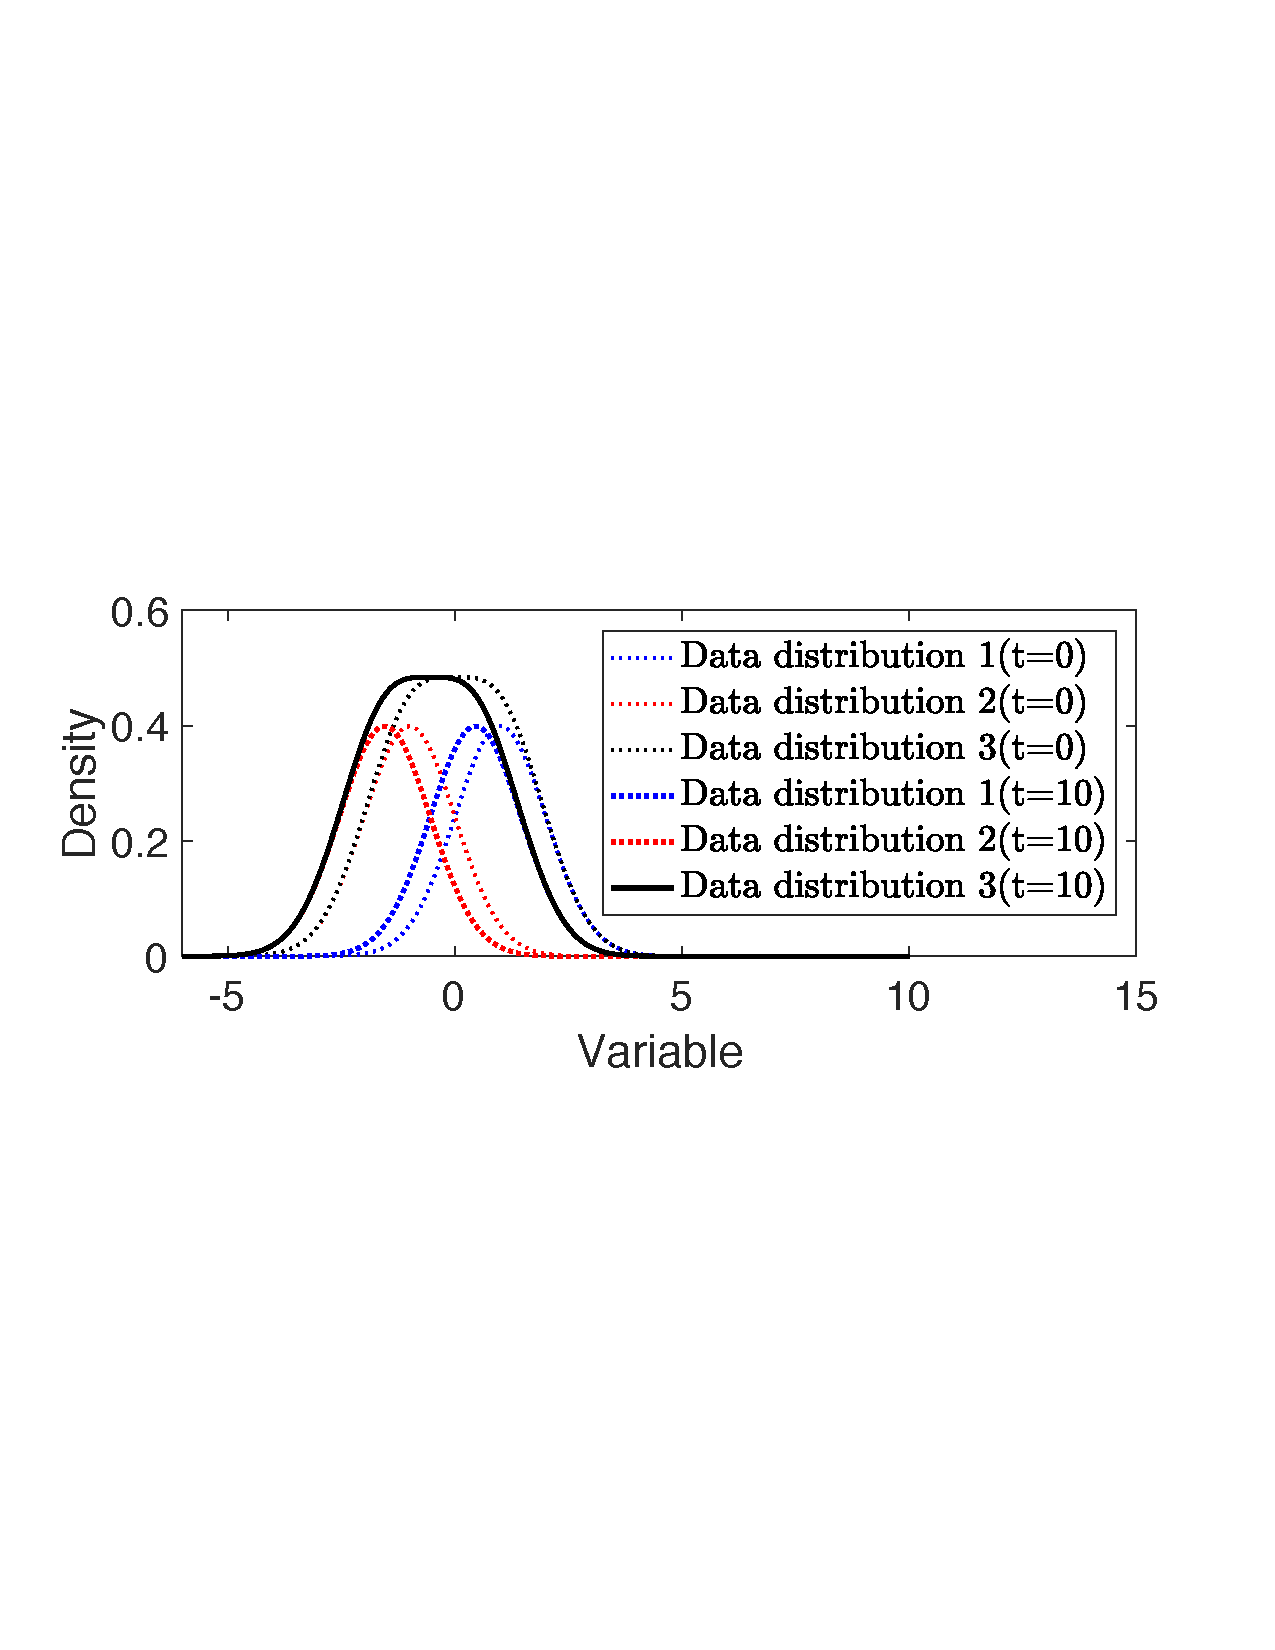
\includegraphics[width=0.7\columnwidth]{figure_dynamics}\label{figure_dynamics}}
\caption{An illustration of the dynmaics caused by the time-varying distributions of data. Data distributions $1$ and $2$ satisify $N(1+\sin(t), 1)$ and $N(-1+\sin(t), 1)$, respectively. Data distribution $3$ is the sum of them, which changes over time. }
\label{figure_illus_dynamics}
\end{figure}


\begin{figure*}[!h]
\setlength{\abovecaptionskip}{0pt}
\setlength{\belowcaptionskip}{0pt}
\centering 
\subfigure[\textit{synthetic data}, $100$ nodes]{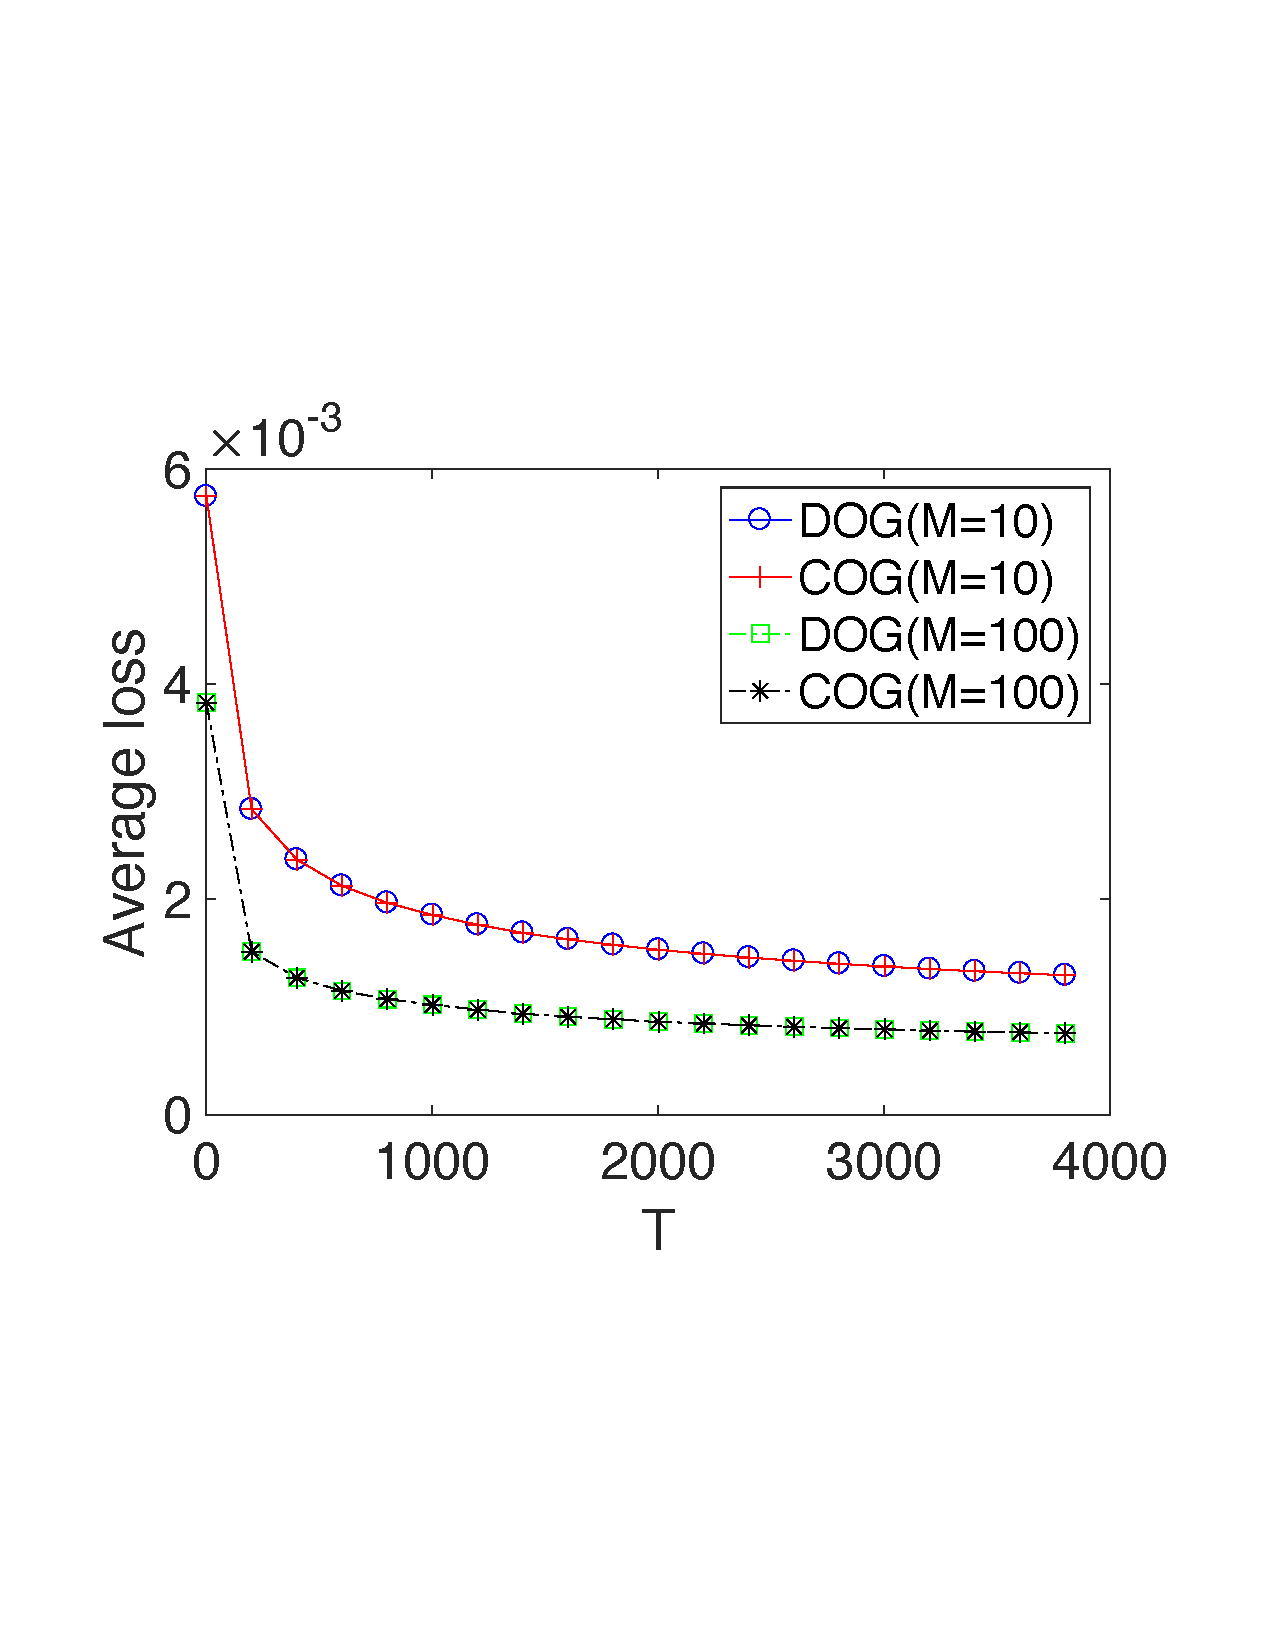
\includegraphics[width=0.48\columnwidth]{figure_decen_cen_ave_loss_iterations}\label{figure_decen_cen_ave_loss_iterations}}
\subfigure[\textit{room-occupancy}, $5$ nodes]{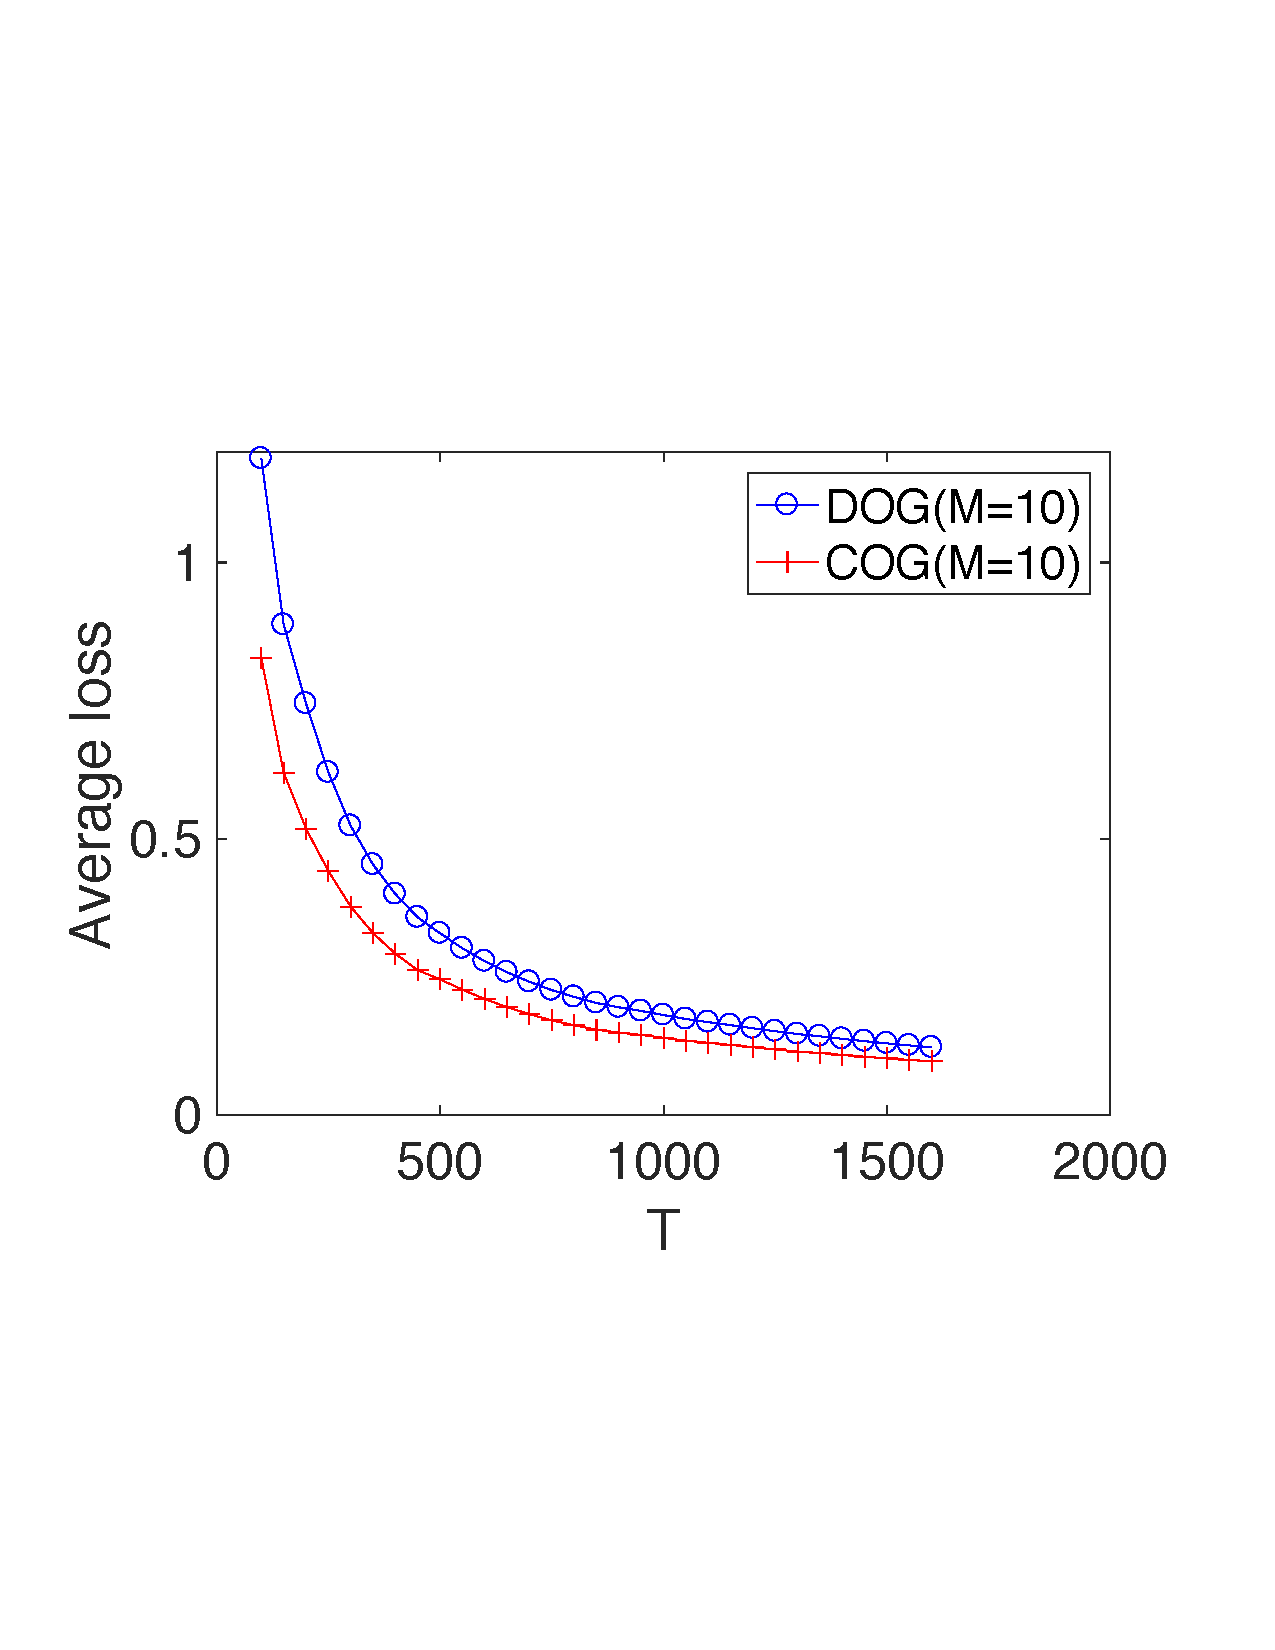
\includegraphics[width=0.48\columnwidth]{figure_decen_cen_ave_loss_iterations_occupancy}\label{figure_decen_cen_ave_loss_iterations_occupancy}}
\subfigure[\textit{usenet2}, $5$ nodes]{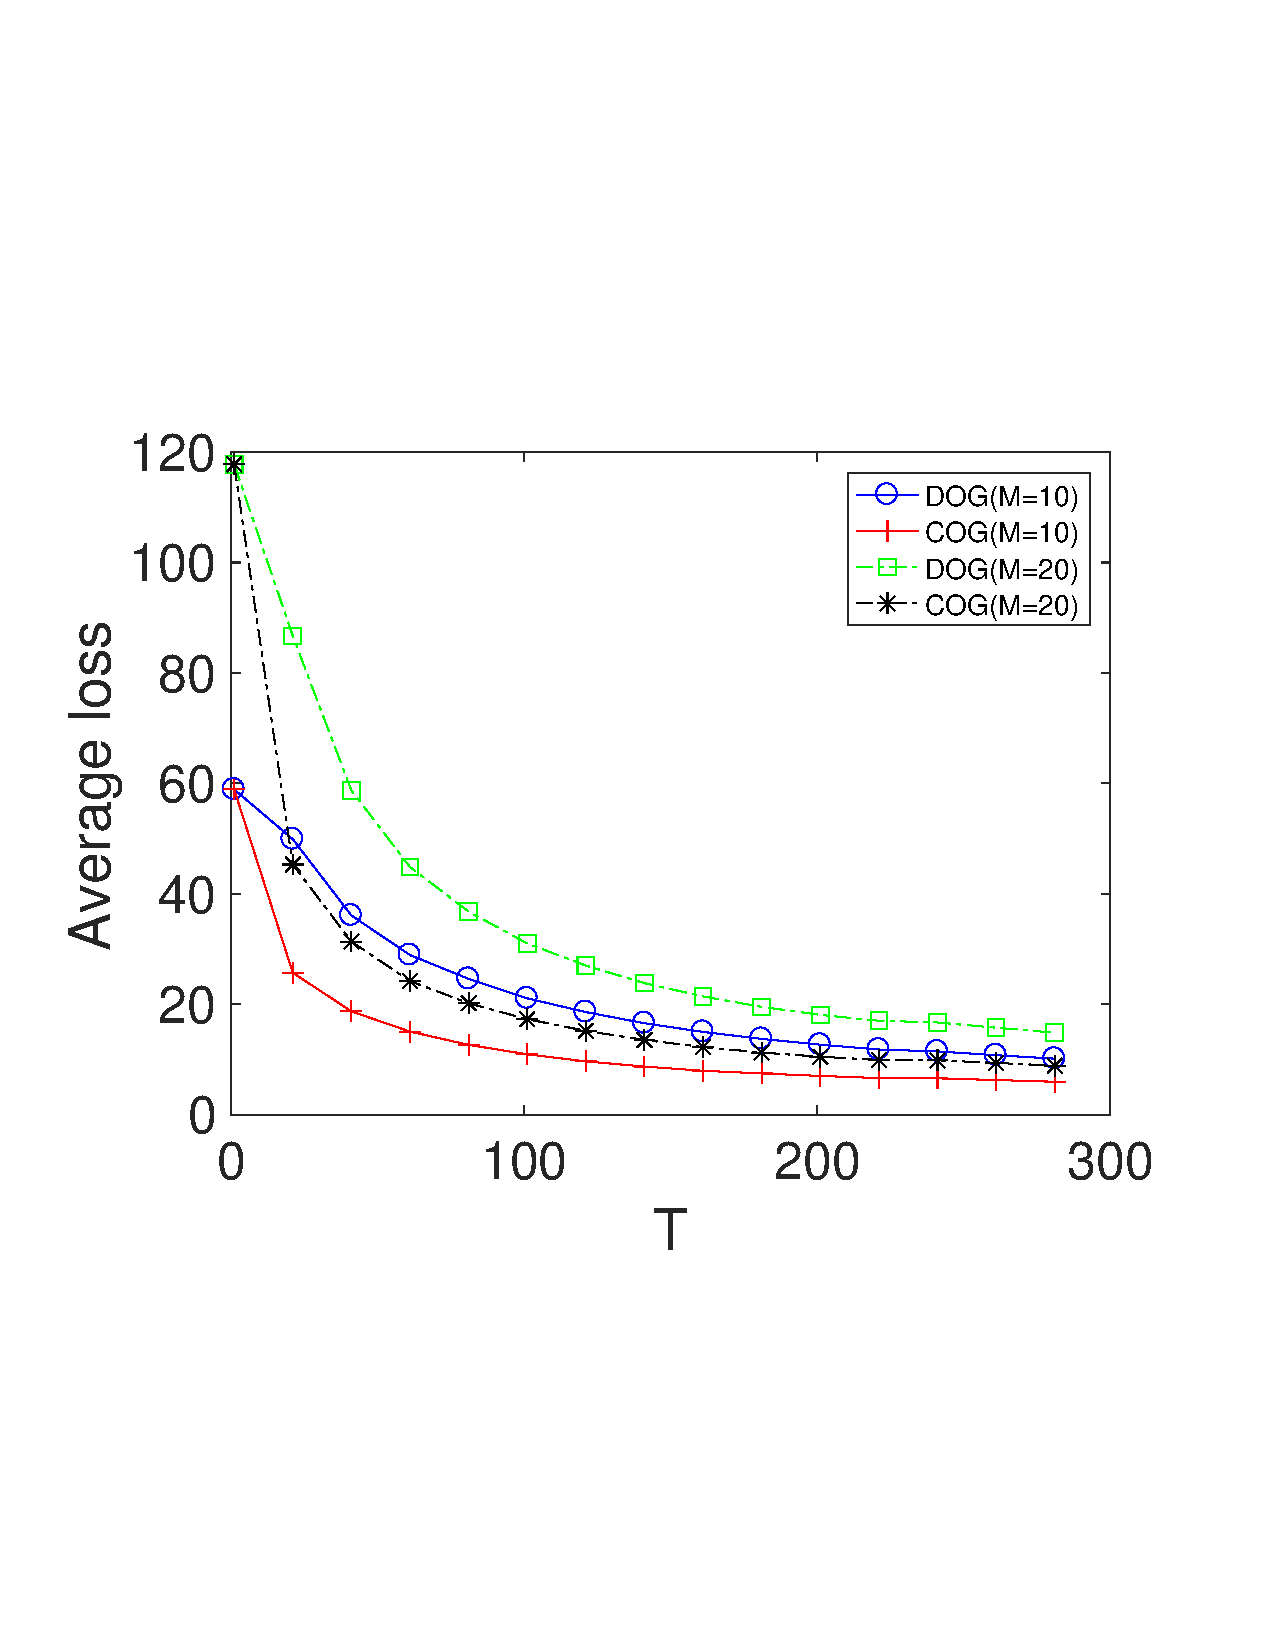
\includegraphics[width=0.48\columnwidth]{figure_decen_cen_ave_loss_iterations_usenet2}\label{figure_decen_cen_ave_loss_iterations_usenet2}}
\subfigure[\textit{spam}, $5$ nodes]{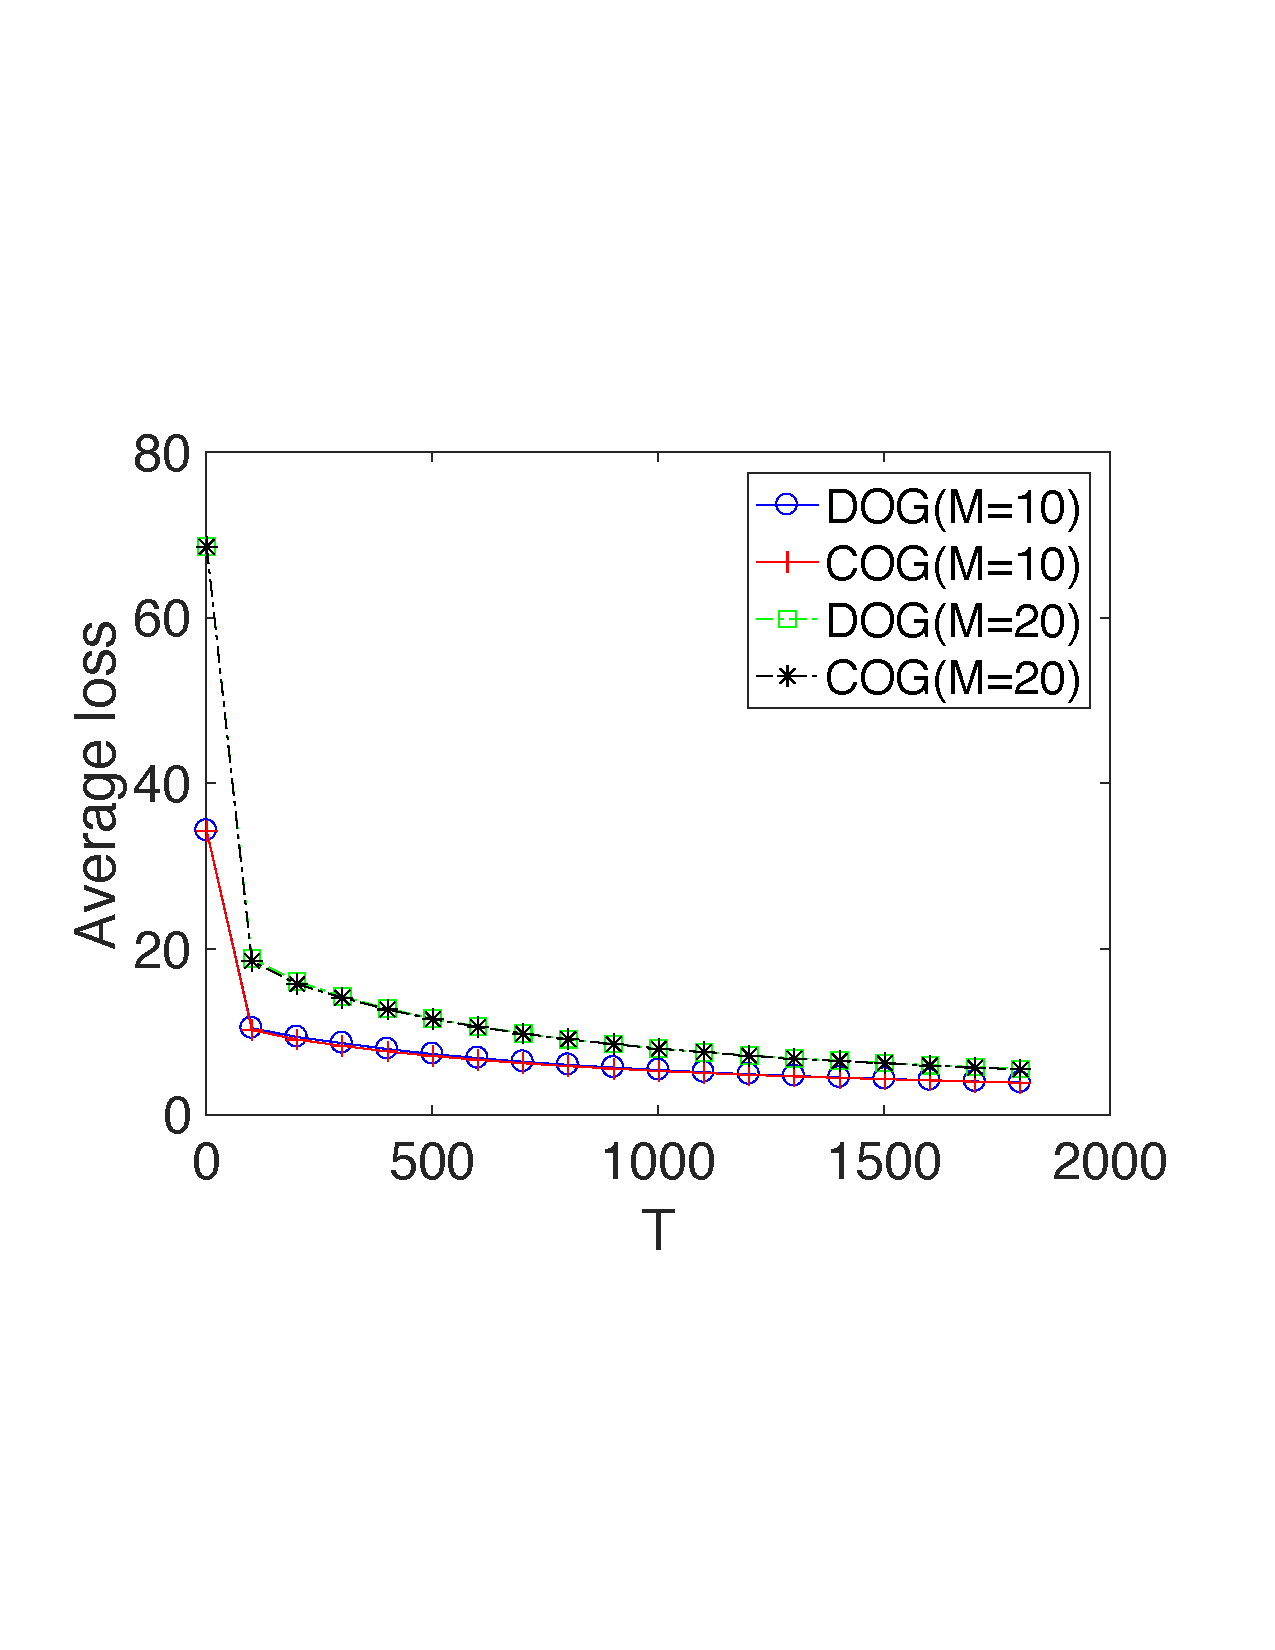
\includegraphics[width=0.48\columnwidth]{figure_decen_cen_ave_loss_iterations_spam}\label{figure_decen_cen_ave_loss_iterations_spam}}
%\subfigure[\textit{usenet2}]{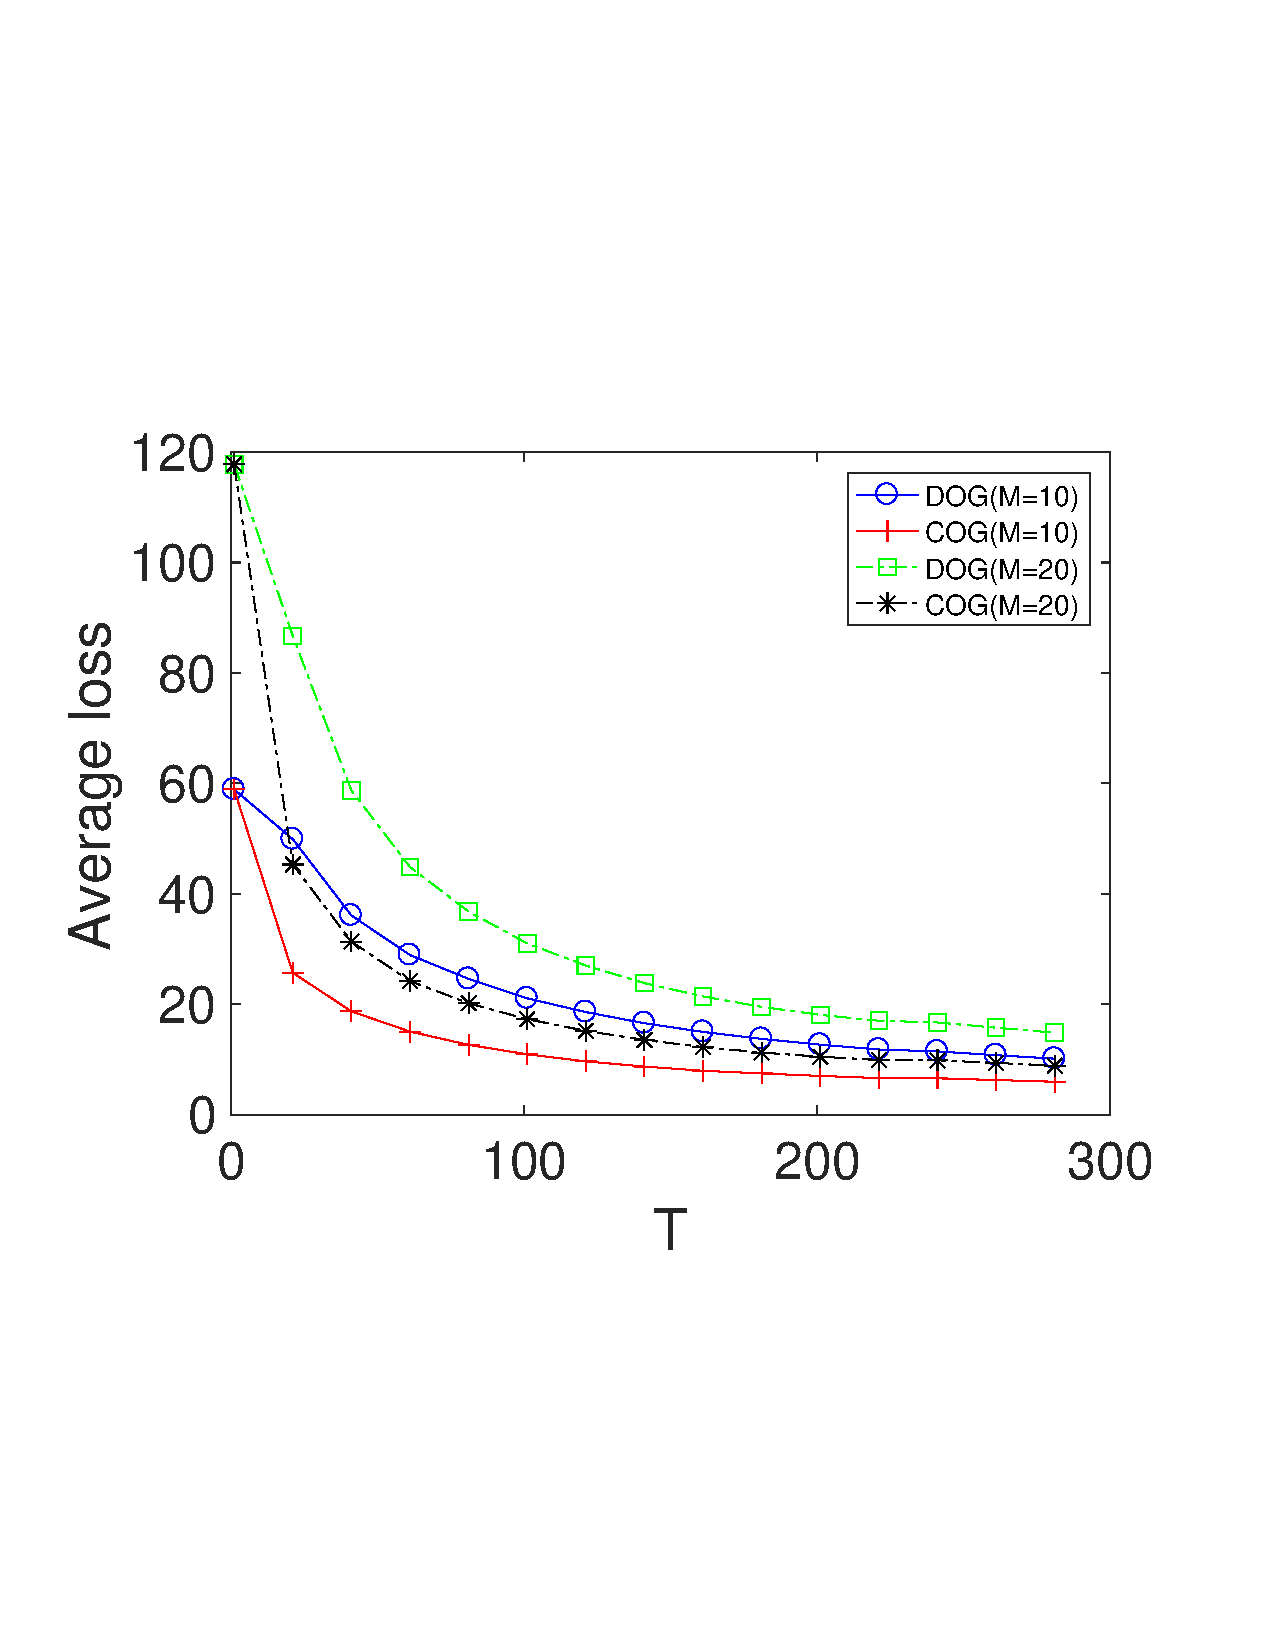
\includegraphics[width=0.32\columnwidth]{figure_decen_cen_ave_loss_iterations_usenet2}\label{figure_decen_cen_ave_loss_iterations_usenet2}}
\caption{The average loss yielded by DOG is comparable to that yielded by COG.}
\label{figure_compare_loss}
\end{figure*}




To test the proposed algorithm, we utilized a toy dataset and three real-world datasets, whose details are as follows.

\textbf{Synthetic Data} 
For the $i$-th node, a data matrix  $\A_i\in R^{10\times T}$ is generated, s.t. $\A_i=0.1\tilde{\A}_i+0.9\hat{\A}_i$, where $\tilde{\A}_i$ represents the adversary part of data, and $\hat{\A}_i$ represents the stochastic part of data. Specifically,  elements of $\tilde{\A}_i$ is uniformly sampled from the interval $[-0.5+\sin(i),0.5+\sin(i)]$. Note that $\tilde{\A}_i$ and $\tilde{\A}_j$ with $i\neq j$ are drawn from different distributions. $\hat{\A}_{i,t}$ is generated according to $\y_{i,t}\in\{1,-1\}$ which is generated uniformly. When $\y_{i,t}=1$, $\hat{\A}_{i,t}$ is generated by sampling from a time-varying distribution $N((1+0.5\sin(t))\cdot\1, \I)$. When $\y_{i,t} = -1$, $\hat{\A}_{i,t}$ is generated by sampling from another time-varying distribution $N((-1+0.5\sin(t))\cdot\1, \I)$. Due to this correlation, $y_{i,t}$ can be considered as the label of the instance $\hat{\A}_{i,t}$.
The above dynamics of time-varying distributions are illustrated in Figure~\ref{figure_illus_dynamics}, which shows the change of the optimal learning model over time and the importance of studying the dynamic regret. 

\textbf{Real Data}
Three real public datasets are \textit{room-occupancy}\footnote{\url{https://archive.ics.uci.edu/ml/datasets/Occupancy+Detection+}},  \textit{usenet2}\footnote{\url{http://mlkd.csd.auth.gr/concept_drift.html}}, and \textit{spam}\footnote{\url{http://mlkd.csd.auth.gr/concept_drift.html}}. \textit{room-occupancy} is a time-series dataset, which is from a natural dynamic enviroment. Both \textit{usenet2} and \textit{spam} are  ``concept drift" \citep{Katakis:2010:TR} datasets, for which the optimal model changes over time.

%Besides, we fetch values of the first feature of every dataset, and then permutate them by the decreasing order. After that, we re-fill the new values to the data matrix to simulate the adversary values. Finally, all values of a feature have been normalized to be zero mean and one variance.
%\begin{itemize}
%\item {\textit{room-occupancy}.} It collects features of a room including temperature, humidity, light, and CO2 for every minute between 02/02/2015 and 02/10/2015. Label of an instance is whether the room is occupied. Our goal is to learn a classification model to make a decision whether the room is occupied by using those features.   
%\item {\textit{usenet2}.} It is an online retail dataset, which contains all transactions occurring between 01/12/2010 and 09/12/2011 for a UK-based and registered non-store online retail. We use three features, that is, \textit{whether a transaction is cancelled}, \textit{quantity}, and \textit{unit price}. We need to train a binary clssification model to make a decision whether a customer is coming from United Kingdom. 
%\item {\textit{BeijingPM2.5}.} It collects some weather features, e.g., teperature and pressure, and the PM2.5 data of US Embassy in Beijing hourly between 01/01/2010 and 12/31/2014. When the PM 2.5 index is larger than $100$, the air quality is \textit{bad}, otherwise, \textit{good}. We want to train a binary clssification model to make a decision whether the air quality is good accoring to features such as temperature and pressure.   \textit{BeijingPM2.5}\footnote{\url{https://archive.ics.uci.edu/ml/datasets/Beijing+PM2.5+Data}},
%\item {\textit{spam}.} Every instance in the dataset is an email, where the frequence of every word in the dictionary is collected. But, the distribution of words changes over time, which is denoted by \textit{concept drift} \citep{Katakis:2010:TR}. We want to learn a classification model to make a decision whether an email is a spam. 
%\end{itemize}


\subsection{Results}

First, figure~\ref{figure_compare_loss} summarizes the performance of DOG compared with COG on all the datasets. 
For the synthetic dataset, we simulated a decentralized network consisting of $100$ nodes; 
For the three real datasets, we simulated a network consisting of $5$ nodes. 
In these networks, the nodes are connected by a ring topology. 
Under these settings, we can observe that both DOG and COG are effective for the online learning tasks on all the datasets, while DOG achieves slightly worse performance. 


{\color{red}
Second, Figure~\ref{figure_compare_network_size} summarizes the effect of the network size on the performance of DOG. We change the number of nodes from $XXX$ to $YYY$ and test on four datasets using the ring topology. Figures~\ref{figure_compare_network_size} draws the curves of average loss over time steps. We observe that the average loss curves are mostly overlapped with different nodes. It shows that DOG is robust to the network size (or number of users), which validates our theory, that is, the average regret does not increase with the number of nodes. 
}

\begin{figure*}[!h]
\setlength{\abovecaptionskip}{0pt}
\setlength{\belowcaptionskip}{0pt}
\centering 
\subfigure[\textit{synthetic data}, ring topology]{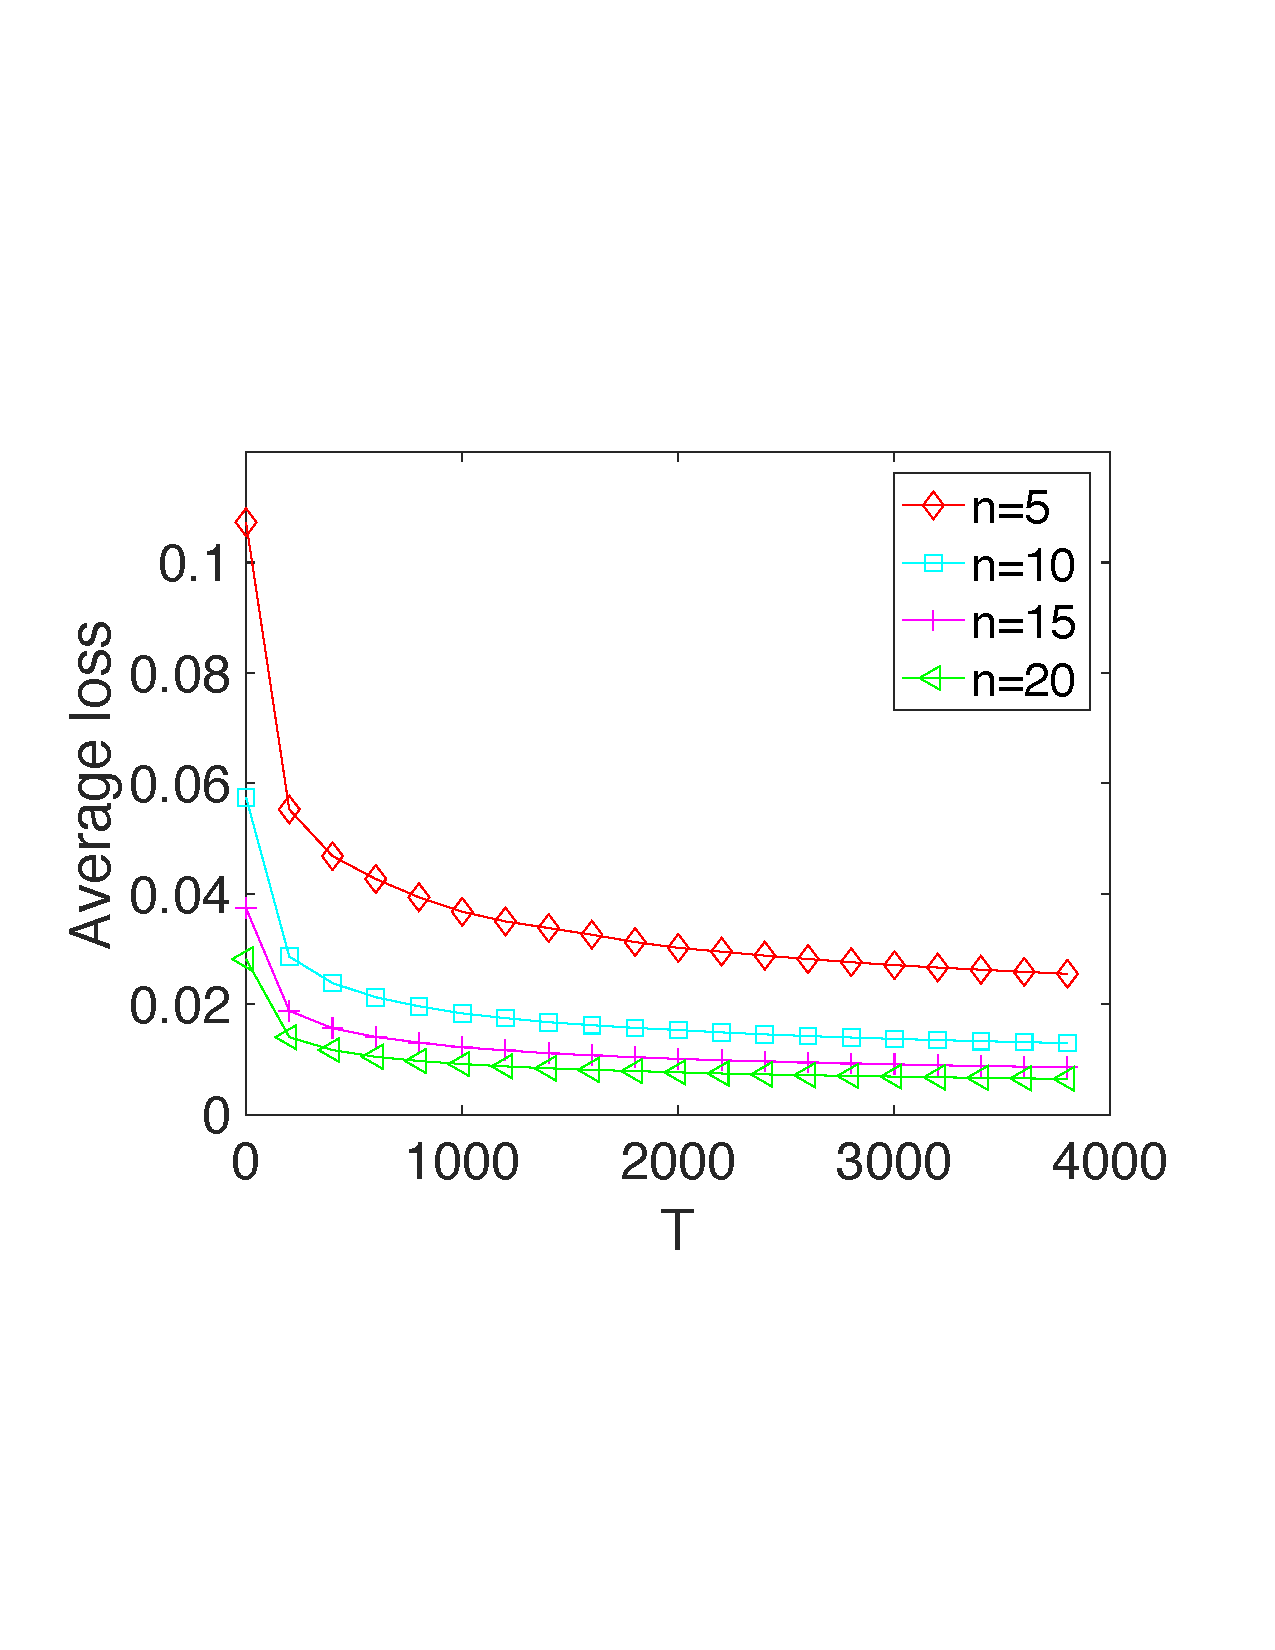
\includegraphics[width=0.48\columnwidth]{figure_decen_cen_ave_loss_nodes}\label{figure_decen_cen_ave_loss_nodes}}
\subfigure[\textit{room-occupancy}, ring topology]{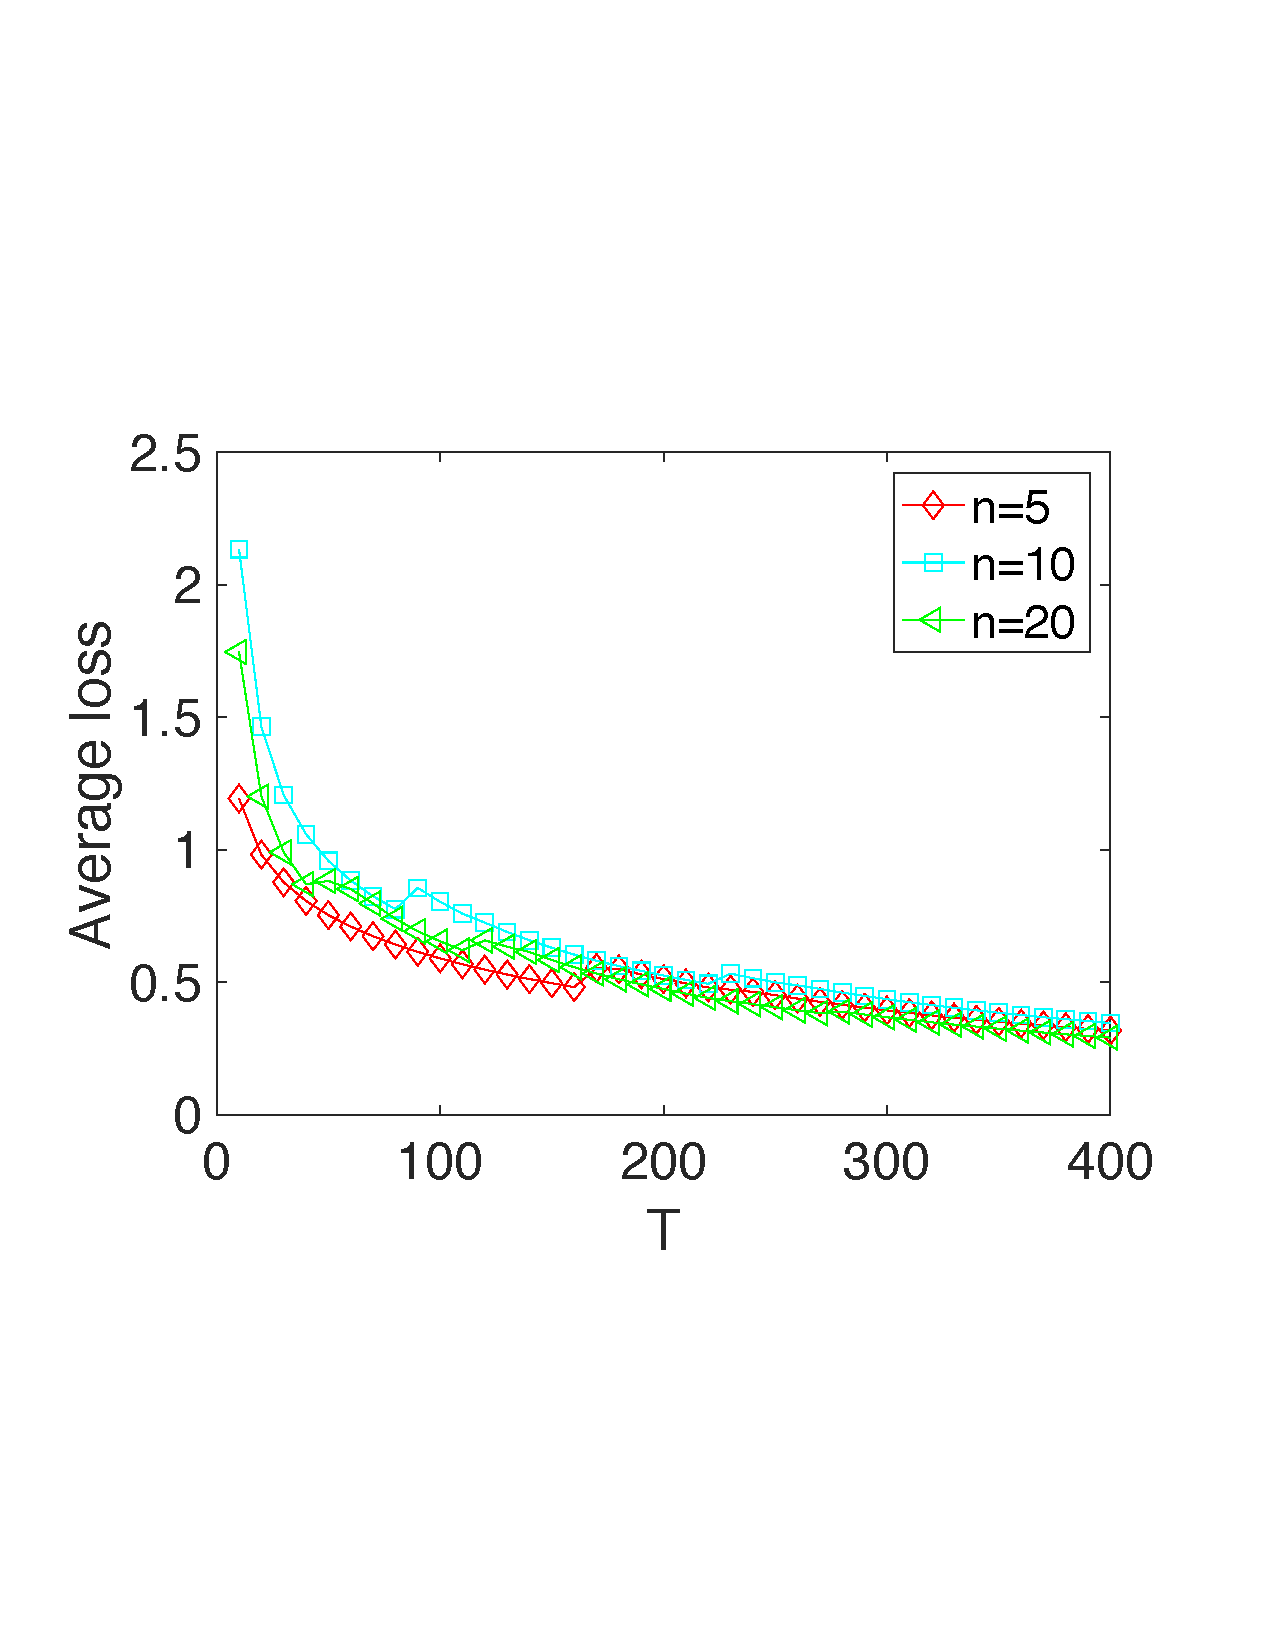
\includegraphics[width=0.48\columnwidth]{figure_decen_cen_ave_loss_nodes_occupancy}\label{figure_decen_cen_ave_loss_nodes_occupancy}}
\subfigure[\textit{usenet2}, ring topology]{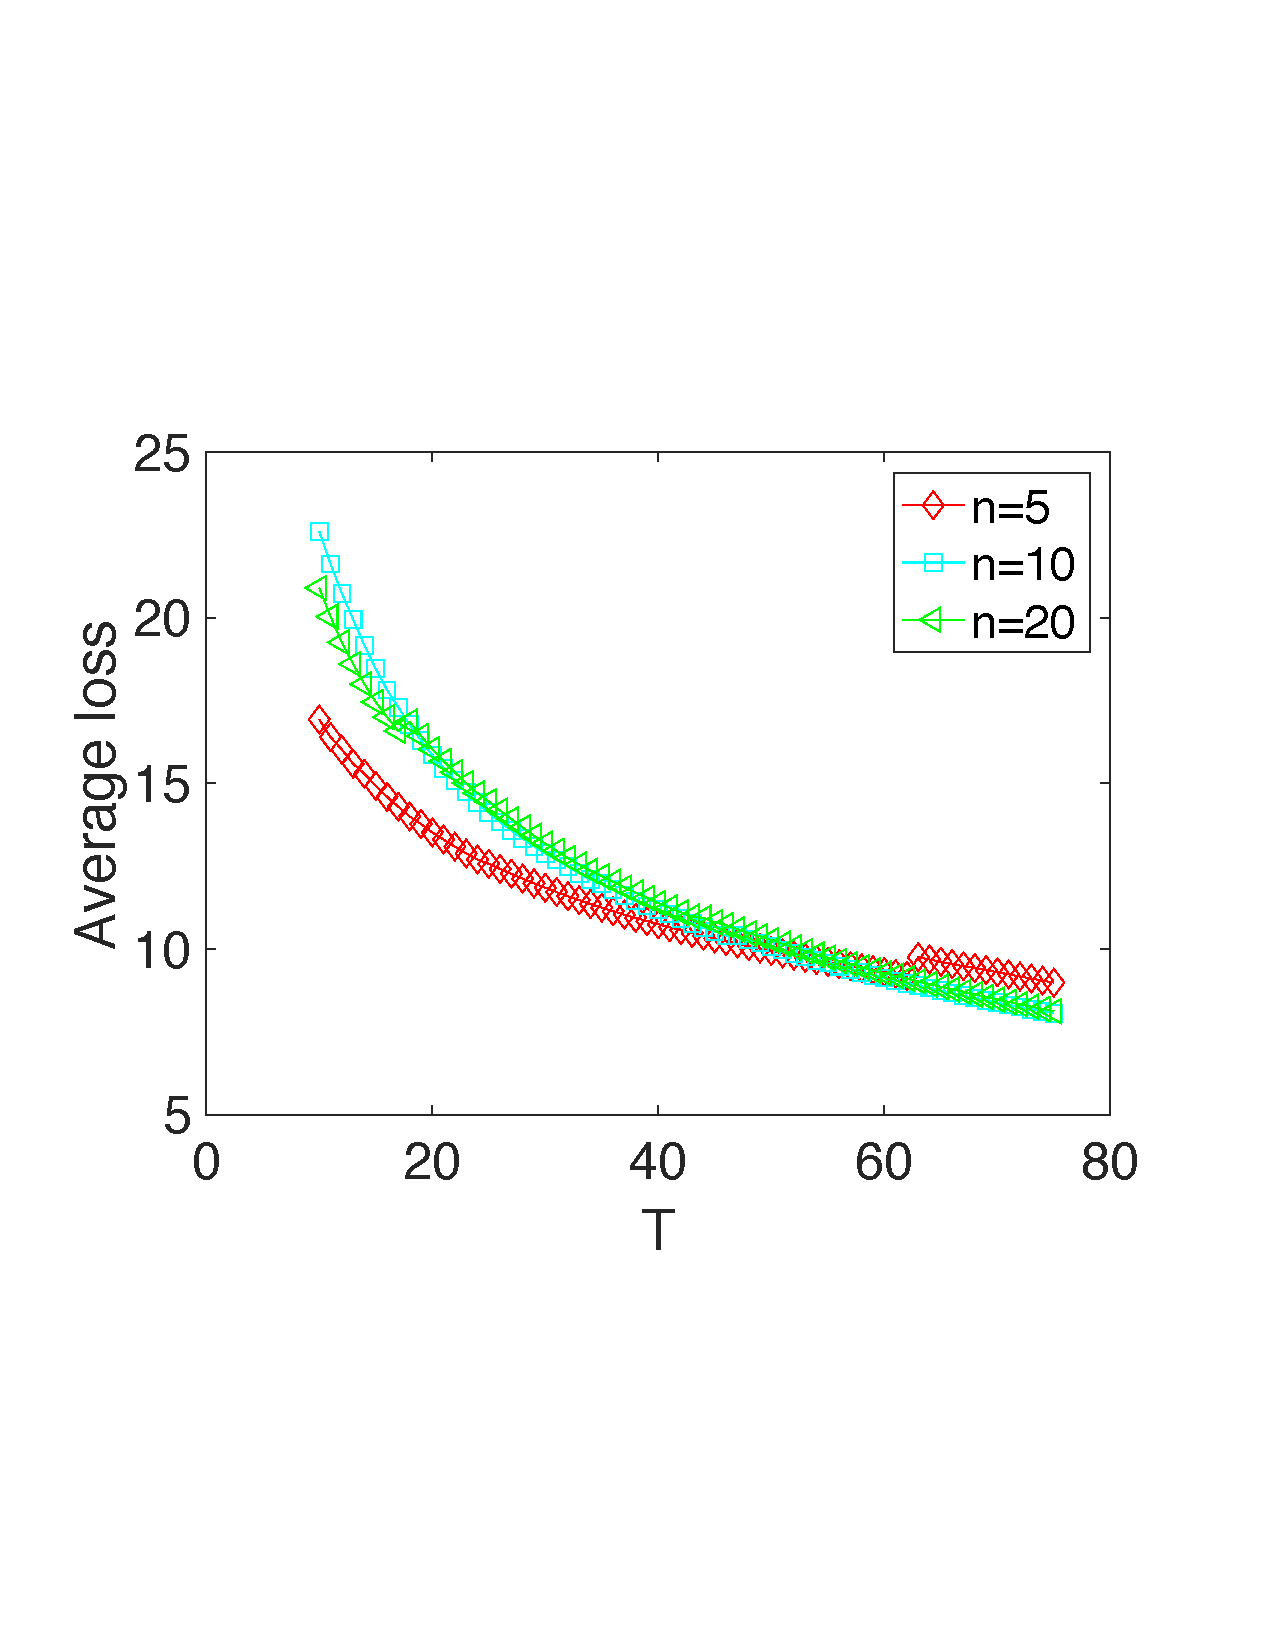
\includegraphics[width=0.48\columnwidth]{figure_decen_cen_ave_loss_nodes_usenet2}\label{figure_decen_cen_ave_loss_nodes_usenet2}}
\subfigure[\textit{spam}, ring topology]{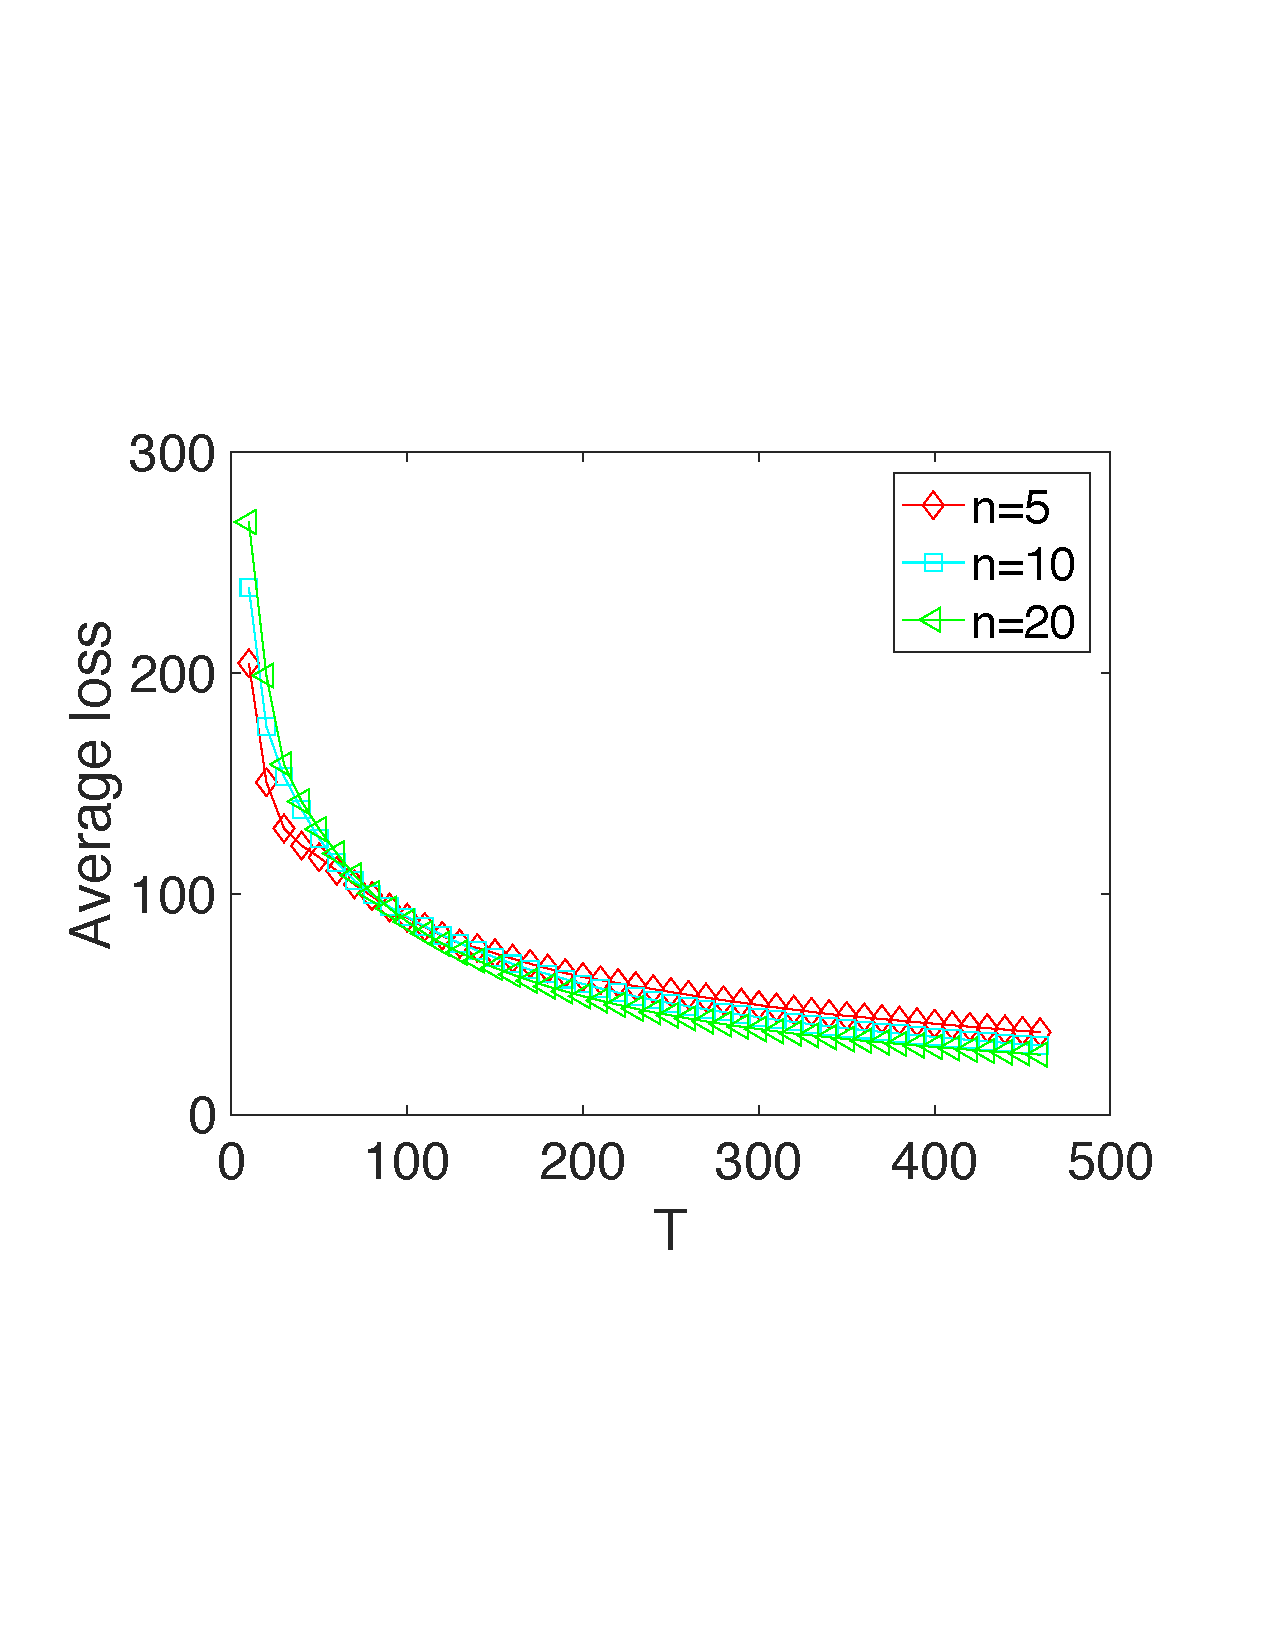
\includegraphics[width=0.48\columnwidth]{figure_decen_cen_ave_loss_nodes_spam}\label{figure_decen_cen_ave_loss_nodes_spam}}
\caption{The average loss yielded by DOG is insensitive to the network size.}
\label{figure_compare_network_size}
\end{figure*}


Third, figure~\ref{figure_compare_topology} shows the effect of the topology of the network on the performance of DOG, for which four different topologies are used. Besides the ring topology, the \textit{Fully connected} means all nodes are connected, where DOG de-generates to be COG. The topology  \textit{WattsStrogatz} represents a Watts-Strogatz small-world graph, for which we can use a parameter to control the number of random edges (set as $0.5$ and $1$ in this paper). The result shows \textit{Fully connected} enjoyes the best performance, because that $\rho = 0$ for it while $\rho>0$ for other topologies.  



\begin{figure*}[!h]
\setlength{\abovecaptionskip}{0pt}
\setlength{\belowcaptionskip}{0pt}
\centering 
\subfigure[\textit{synthetic data}, $100$ nodes]{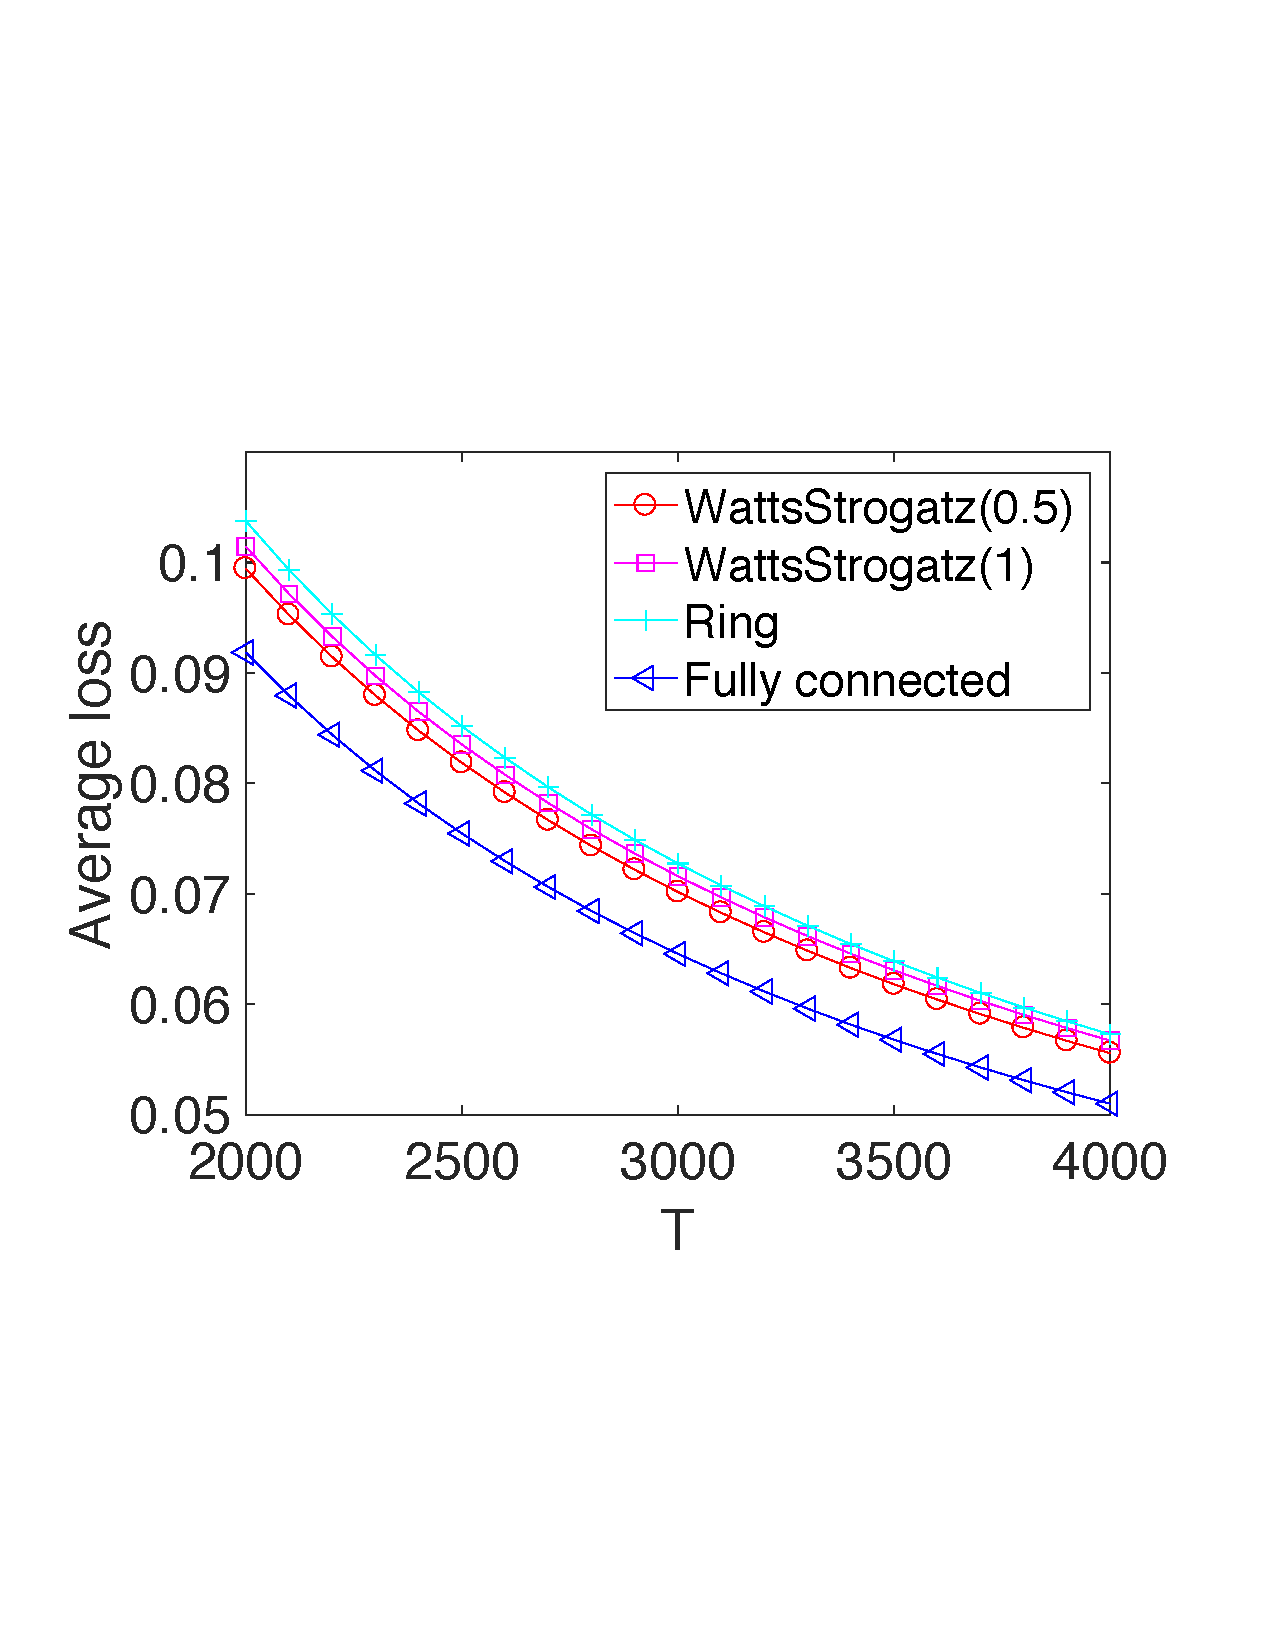
\includegraphics[width=0.48\columnwidth]{figure_decen_cen_ave_loss_iterations_net_types}\label{figure_decen_cen_ave_loss_iterations_net_types}}
\subfigure[\textit{room-occupancy}, $20$ nodes]{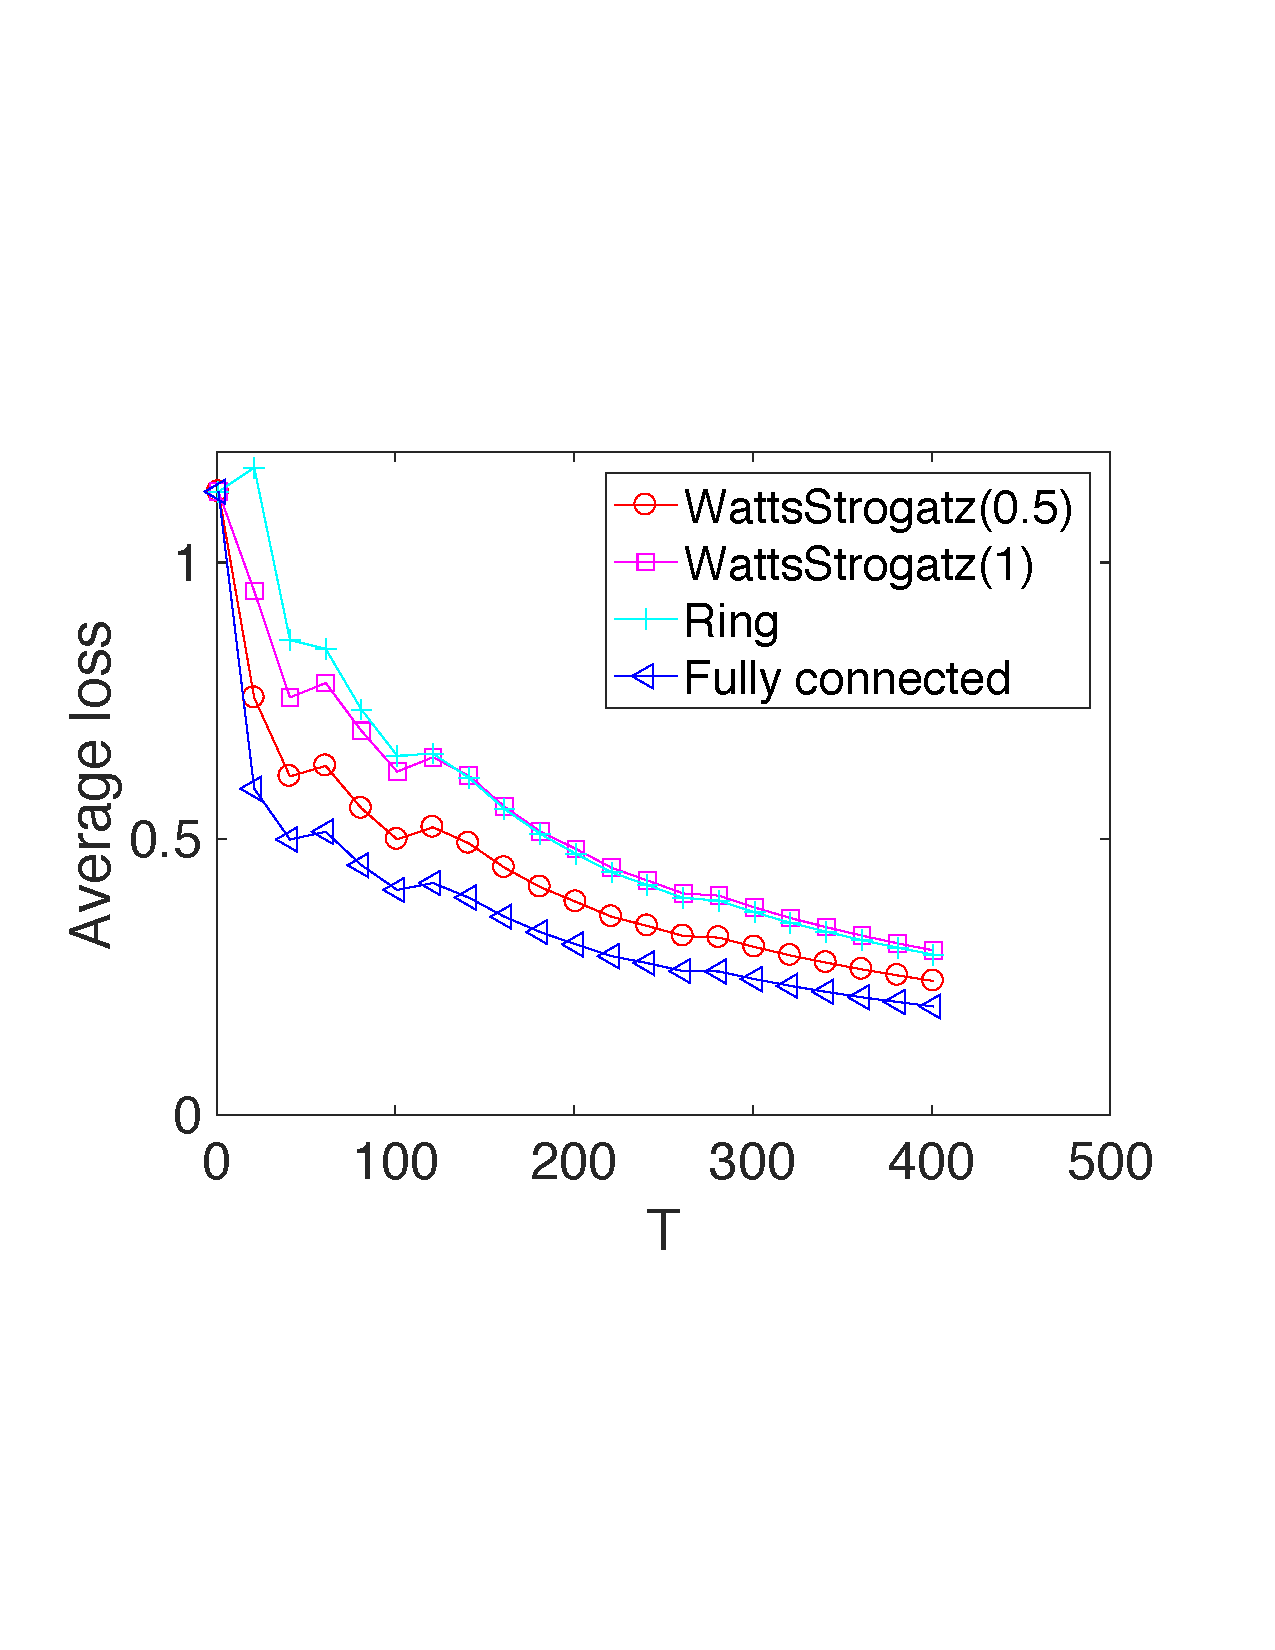
\includegraphics[width=0.48\columnwidth]{figure_decen_cen_ave_loss_iterations_net_types_occupancy}\label{figure_decen_cen_ave_loss_iterations_net_types_occupancy}}
\subfigure[\textit{usenet2}, $20$ nodes]{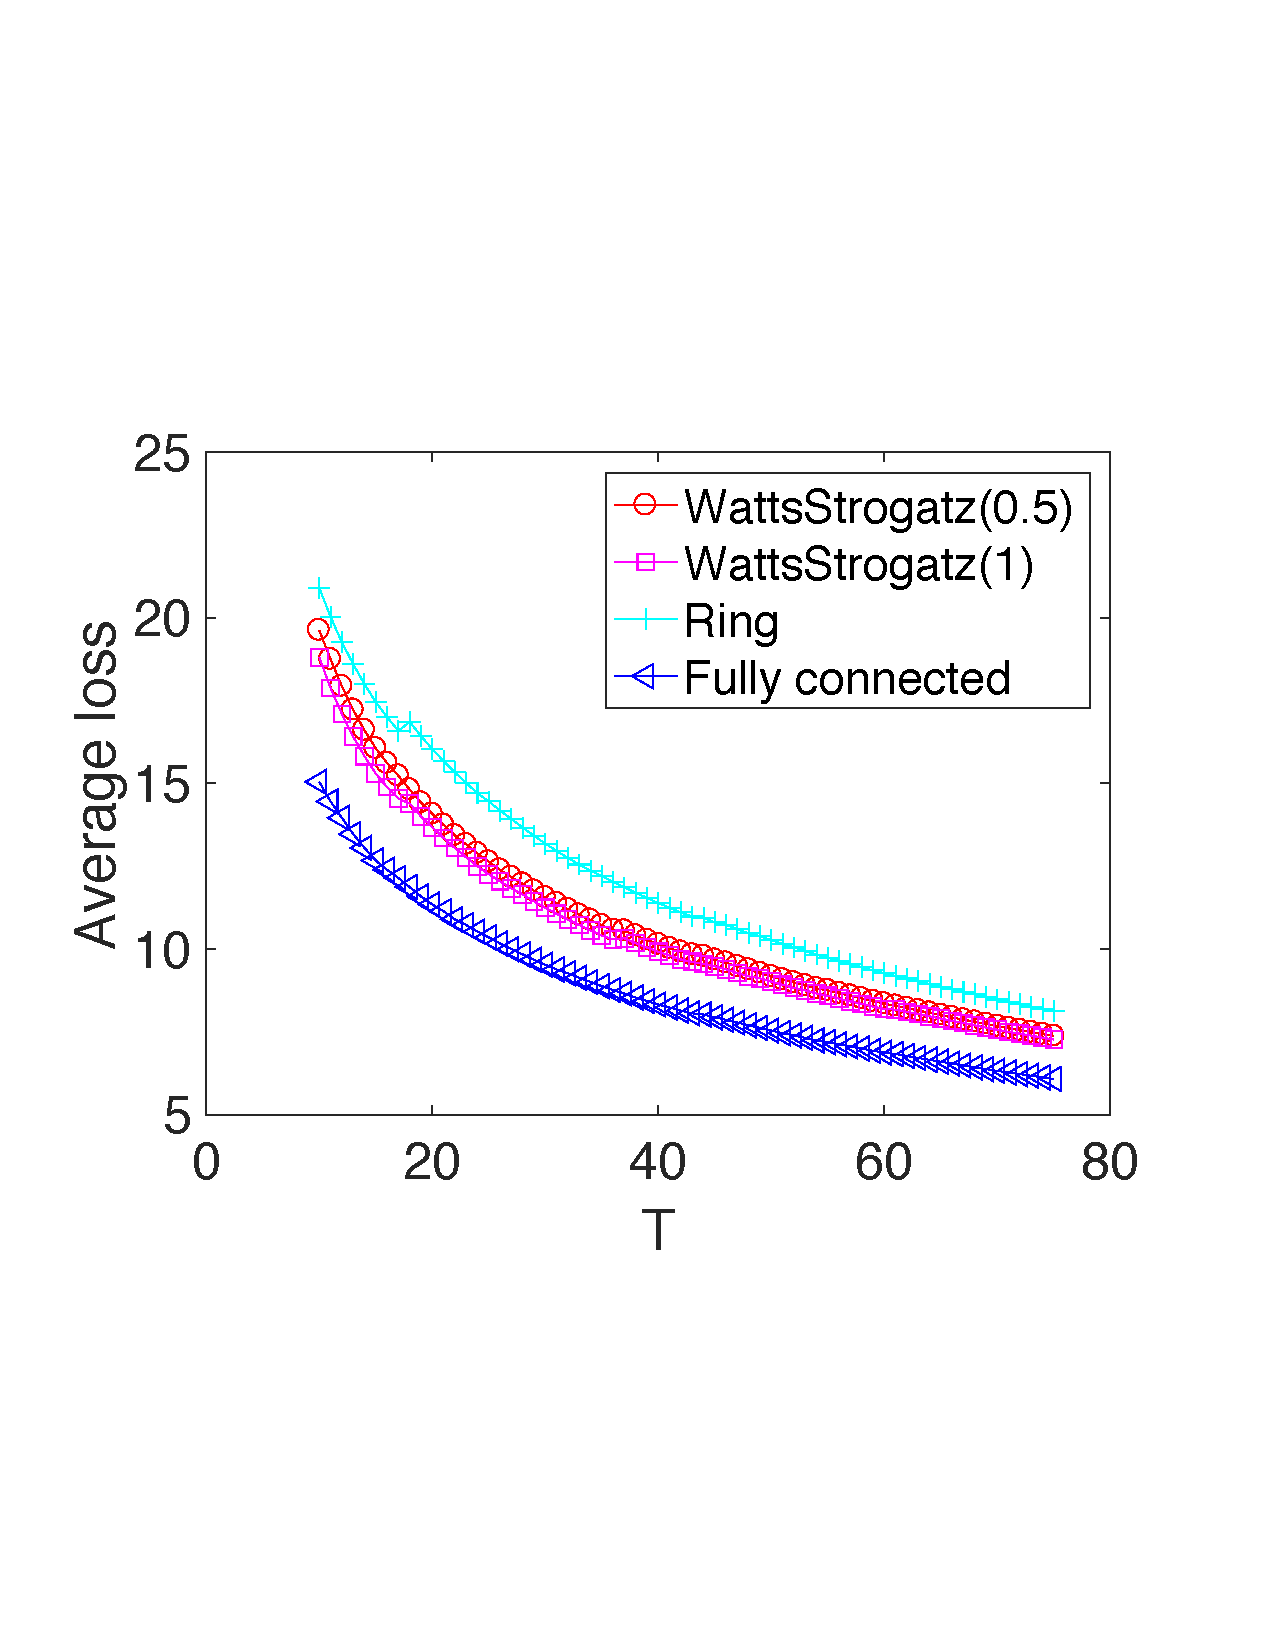
\includegraphics[width=0.48\columnwidth]{figure_decen_cen_ave_loss_iterations_net_types_usenet2}\label{figure_decen_cen_ave_loss_iterations_net_types_occupancy}}
\subfigure[\textit{spam}, $20$ nodes]{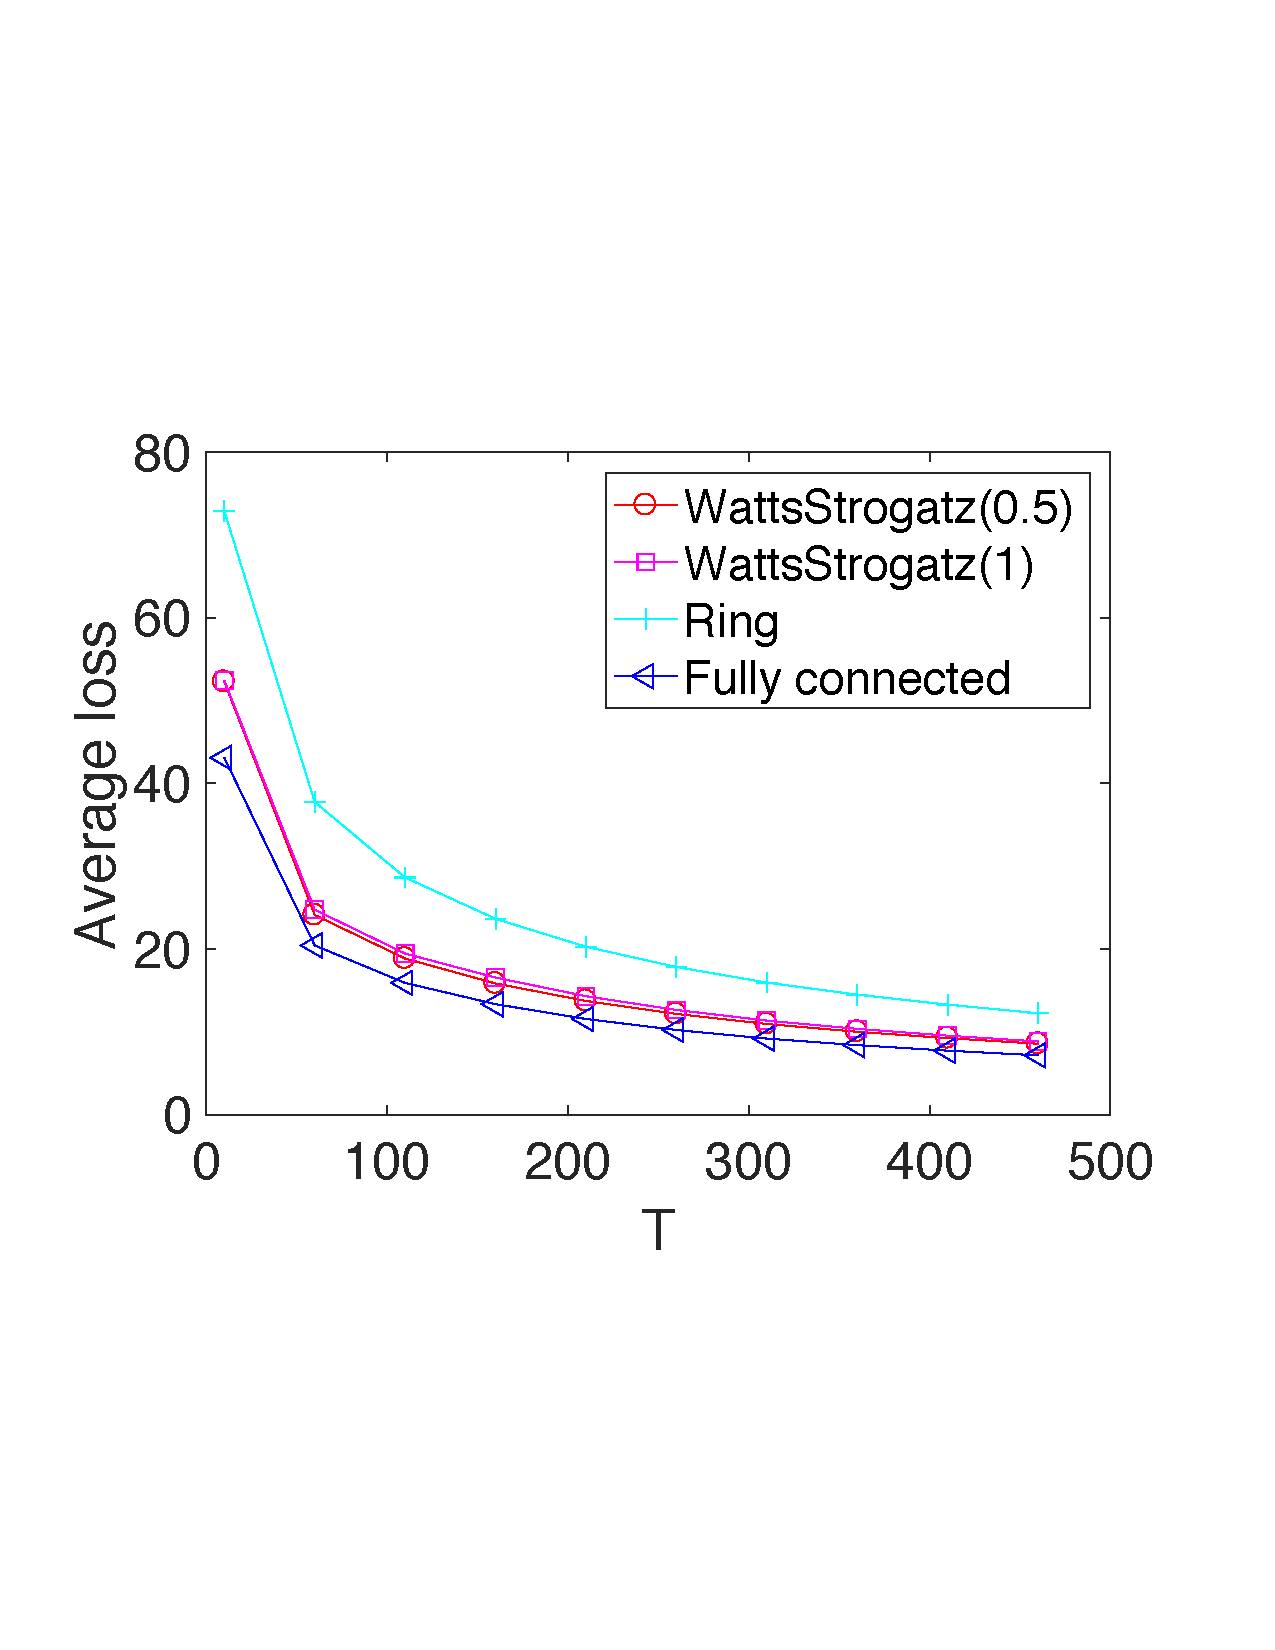
\includegraphics[width=0.48\columnwidth]{figure_decen_cen_ave_loss_iterations_net_types_spam}\label{figure_decen_cen_ave_loss_iterations_net_types_spam}}
\caption{The average loss yielded by DOG is insensitive to the topology of the network.}
\label{figure_compare_topology}
\end{figure*}



\section{Conclusion}
We investigate a new online learning problem in a decentralized network, where the loss incurs by both adversary and stochastic data.  We provide a new analysis framework, which achieves sublinear regret. Extensive empirical studies varify the theoretical result. 


%\section*{References}
\bibliography{reference}

\bibliographystyle{abbrvnat}

\onecolumn

\section*{Appendix}

\textbf{Proof to Theorem \ref{theorem_regret_upper_bound}:}
\begin{proof}
\begin{align}
\nonumber
& \EE_{ \Xi_{n,t} \sim \Dcal_{n,t} } \frac{1}{n}\sum_{i=1}^n f_{i,t}(\x_{i,t};\xi_{i,t}) - f_{i,t}(\x_t^\ast;\xi_{i,t}) \\ \nonumber
\le & \EE_{ \Xi_{n,t} \sim \Dcal_{n,t} } \frac{1}{n}\sum_{i=1}^n \lrangle{ \nabla f_{i,t}(\x_{i,t};\xi_{i,t}),  \x_{i,t} - \x_t^\ast } \\ \nonumber
= & \underbrace{ \EE_{ \Xi_{n,t} \sim \Dcal_{n,t} } \frac{1}{n}\sum_{i=1}^n   \lrincir{\lrangle{\nabla  f_{i,t}(\x_{i,t};\xi_{i,t}), \x_{i,t} - \bar{\x}_t } + \lrangle{\nabla  f_{i,t}(\x_{i,t};\xi_{i,t}), \bar{\x}_t - \bar{\x}_{t+1} } } }_{I_1(t)} \\ \nonumber 
&+ \underbrace{ \EE_{ \Xi_{n,t} \sim \Dcal_{n,t} } \lrangle{\frac{1}{n}\sum_{i=1}^n\nabla f_{i,t}(\x_{i,t};\xi_{i,t}), \bar{\x}_{t+1} - \x_t^\ast } }_{I_2(t)}\\ \nonumber
\end{align}

Now, we begin to bound $I_1(t)$.
\begin{align}
\nonumber
I_1(t) = &    \lrincir{\underbrace{ \EE_{ \Xi_{n,t} \sim \Dcal_{n,t} }\frac{1}{n}\sum_{i=1}^n\lrangle{\nabla f_{i,t}(\x_{i,t}; \xi_{i,t}), \x_{i,t} - \bar{\x}_t } }_{J_1(t)} +  \underbrace{ \EE_{ \Xi_{n,t} \sim \Dcal_{n,t} }\lrangle{\frac{1}{n}\sum_{i=1}^n \nabla f_{i,t}(\x_{i,t};\xi_{i,t}), \bar{\x}_t - \bar{\x}_{t+1} }}_{J_2(t)}}.
\end{align} For $J_1(t)$, we have
\begin{align}
\nonumber
& J_1(t) \\ \nonumber 
= & \frac{1}{n}\EE_{ \Xi_{n,t} \sim \Dcal_{n,t} }\sum_{i=1}^n\lrangle{\nabla f_{i,t}(\x_{i,t}; \xi_{i,t}), \x_{i,t} - \bar{\x}_t } \\ \nonumber
= & \frac{1}{n}\EE_{ \Xi_{n,t} \sim \Dcal_{n,t} } \sum_{i=1}^n\lrangle{\nabla f_{i,t}(\x_{i,t}; \xi_{i,t}) - \nabla F_{i,t}(\bar{\x}_t), \x_{i,t} - \bar{\x}_t } + \frac{1}{n}\EE_{ \Xi_{n,t-1} \sim \Dcal_{t-1} }\sum_{i=1}^n\lrangle{\nabla F_{i,t}(\bar{\x}_t), \x_{i,t} - \bar{\x}_t } \\ \nonumber
= & \frac{1}{n}\EE_{ \Xi_{n,t-1} \sim \Dcal_{t-1} }\sum_{i=1}^n\lrangle{\nabla F_{i,t}(\x_{i,t}) - \nabla F_{i,t}(\bar{\x}_t), \x_{i,t} - \bar{\x}_t } + \EE_{ \Xi_{n,t-1} \sim \Dcal_{t-1} }\lrangle{\nabla F_{i,t}(\bar{\x}_t), \frac{1}{n}\sum_{i=1}^n\x_{i,t} - \bar{\x}_t } \\ \nonumber
\refabovecir{\le}{\textcircled{1}} & \frac{L}{n}\EE_{ \Xi_{n,t-1} \sim \Dcal_{t-1} }\sum_{i=1}^n \lrnorm{\x_{i,t} - \bar{\x}_t}^2。. 
\end{align} $\textcircled{1}$ holds due to $F_{i,t}$ has $L$-Lipschitz gradients, and $\bar{\x}_t = \frac{1}{n}\sum_{i=1}^n \x_{i,t}$.

For $J_2(t)$, we have
\begin{align}
\nonumber
& J_2(t) \\ \nonumber 
= & \EE_{ \Xi_{n,t} \sim \Dcal_{n,t} }\lrangle{\frac{1}{n}\sum_{i=1}^n\nabla f_{i,t}(\x_{i,t};\xi_{i,t}), \bar{\x}_t - \bar{\x}_{t+1} } \\ \nonumber
\le & \frac{\eta}{2}\EE_{ \Xi_{n,t} \sim \Dcal_{n,t} } \lrnorm{\frac{1}{n}\sum_{i=1}^n \nabla f_{i,t}(\x_{i,t};\xi_{i,t})}^2 + \frac{1}{2\eta} \EE_{ \Xi_{n,t} \sim \Dcal_{n,t} }\lrnorm{ \bar{\x}_t - \bar{\x}_{t+1}}^2  \\ \nonumber
\le & \frac{\eta}{2}\EE_{ \Xi_{n,t} \sim \Dcal_{n,t} }\lrnorm{\frac{1}{n}\sum_{i=1}^n \lrincir{\nabla  f_{i,t}(\x_{i,t};\xi_{i,t}) - \nabla F_{i,t}(\x_{i,t}) + \nabla F_{i,t}(\x_{i,t})} }^2 + \frac{1}{2\eta} \EE_{ \Xi_{n,t} \sim \Dcal_{n,t} }\lrnorm{ \bar{\x}_t - \bar{\x}_{t+1}}^2  \\ \nonumber
\le &  \eta\EE_{ \Xi_{n,t} \sim \Dcal_{n,t} }\lrnorm{\frac{1}{n}\sum_{i=1}^n \lrincir{ \nabla f_{i,t}(\x_{i,t};\xi_{i,t}) - \nabla F_{i,t}(\x_{i,t}) } }^2 + \eta \EE_{ \Xi_{n,t-1} \sim \Dcal_{t-1} }\lrnorm{\frac{1}{n}\sum_{i=1}^n\nabla F_{i,t}(\x_{i,t})}^2 \\ \nonumber 
& + \frac{1}{2\eta} \EE_{ \Xi_{n,t} \sim \Dcal_{n,t} }\lrnorm{ \bar{\x}_t - \bar{\x}_{t+1}}^2  \\ \nonumber
\refabovecir{\le}{\textcircled{1}} & \frac{\eta}{n} \sigma^2 + \eta \EE_{ \Xi_{n,t-1} \sim \Dcal_{t-1} }\lrnorm{ \frac{1}{n}\sum_{i=1}^n \lrincir{ \nabla F_{i,t}(\x_{i,t}) - \nabla F_{i,t}(\bar{\x}_t) + \nabla F_{i,t}(\bar{\x}_t) } }^2 + \frac{1}{2\eta} \EE_{ \Xi_{n,t} \sim \Dcal_{n,t} }\lrnorm{ \bar{\x}_t - \bar{\x}_{t+1}}^2 \\ \nonumber
\le & \frac{\eta}{n} \sigma^2 + 2\eta \EE_{ \Xi_{n,t-1} \sim \Dcal_{t-1} }\lrnorm{\frac{1}{n}\sum_{i=1}^n \lrincir{ \nabla F_{i,t}(\x_{i,t}) - \nabla F_{i,t}(\bar{\x}_t) } }^2 \\ \nonumber 
& + 2\eta \EE_{ \Xi_{n,t-1} \sim \Dcal_{t-1} }\lrnorm{\nabla F_{i,t}(\bar{\x}_t)}^2 + \frac{1}{2\eta} \EE_{ \Xi_{n,t} \sim \Dcal_{n,t} }\lrnorm{ \bar{\x}_t - \bar{\x}_{t+1}}^2 \\ \nonumber
\le & \frac{\eta}{n} \sigma^2 + \frac{2\eta}{n} \EE_{ \Xi_{n,t-1} \sim \Dcal_{t-1} }\sum_{i=1}^n\lrnorm{ \nabla F_{i,t}(\x_{i,t}) - \nabla F_{i,t}(\bar{\x}_t)  }^2 \\ \nonumber 
& + 2\eta \EE_{ \Xi_{n,t-1} \sim \Dcal_{t-1} }\lrnorm{\nabla F_{i,t}(\bar{\x}_t)}^2 + \frac{1}{2\eta} \EE_{ \Xi_{n,t} \sim \Dcal_{n,t} }\lrnorm{ \bar{\x}_t - \bar{\x}_{t+1}}^2 \\ \nonumber
\refabovecir{\le}{\textcircled{2}} & \frac{\eta}{n} \sigma^2 + \frac{2\eta L^2}{n}\EE_{ \Xi_{n,t-1} \sim \Dcal_{t-1} }\sum_{i=1}^n \lrnorm{\x_{i,t} - \bar{\x}_t }^2 + 2\eta \EE_{ \Xi_{n,t-1} \sim \Dcal_{t-1} }\lrnorm{\nabla F_{i,t}(\bar{\x}_t)}^2 + \frac{1}{2\eta} \EE_{ \Xi_{n,t} \sim \Dcal_{n,t} }\lrnorm{ \bar{\x}_t - \bar{\x}_{t+1}}^2.
\end{align} $\textcircled{1}$ holds due to
\begin{align}
\nonumber
& \EE_{ \Xi_{n,t} \sim \Dcal_{n,t} }\lrnorm{\frac{1}{n}\sum_{i=1}^n \lrincir{ \nabla f_{i,t}(\x_{i,t};\xi_{i,t}) - \nabla F_{i,t}(\x_{i,t}) } }^2 \\ \nonumber
= & \frac{1}{n^2}\EE_{ \Xi_{n,t-1} \sim \Dcal_{t-1} }\lrincir{ \sum_{i=1}^n \EE_{ \xi_{i,t} \sim D_{i,t} }\lrnorm{ \nabla f_{i,t}(\x_{i,t};\xi_{i,t}) - \nabla F_{i,t}(\x_{i,t}) }^2  } \\ \nonumber 
& + \frac{1}{n^2}\EE_{ \Xi_{n,t-1} \sim \Dcal_{t-1} }\lrincir{2\sum_{i=1}^n\sum_{j=1, j\neq i}^n\lrangle{ \EE_{ \xi_{i,t} \sim D_{i,t} }\nabla f_{i,t}(\x_{i,t};\xi_{i,t}) - \nabla F_{i,t}(\x_{i,t}),  \EE_{ \xi_{j,t} \sim D_{j,t} } \nabla f_{i,t}(\x_{j,t};\xi_{j,t}) - \nabla F_{j,t}(\x_{j,t})} } \\ \nonumber
= & \frac{1}{n^2}\EE_{ \Xi_{n,t-1} \sim \Dcal_{t-1} }\sum_{i=1}^n \EE_{ \xi_{i,t} \sim D_{i,t} }\lrnorm{ \nabla f_{i,t}(\x_{i,t};\xi_{i,t}) - \nabla F_{i,t}(\x_{i,t}) }^2 + 0 \\ \nonumber
\le & \frac{1}{n} \sigma^2.
\end{align} $\textcircled{2}$ holds due to $F_{i,t}$ has $L$ Lipschitz gradients.

 Therefore, we obtain
\begin{align}
\nonumber
& I_1(t) \\ \nonumber 
= &  (J_1(t) + J_2(t)) \\ \nonumber
= &   \lrincir{ \frac{L}{n}\EE_{ \Xi_{n,t-1} \sim \Dcal_{t-1} }\sum_{i=1}^n \lrnorm{\x_{i,t} - \bar{\x}_t}^2 +\frac{\eta}{n} \sigma^2 + \frac{2\eta L^2}{n}\EE_{ \Xi_{n,t-1} \sim \Dcal_{t-1} }\sum_{i=1}^n \lrnorm{\x_{i,t} - \bar{\x}_t }^2 } \\ \nonumber
& +  \lrincir{ 2\eta \EE_{ \Xi_{n,t-1} \sim \Dcal_{t-1} }\lrnorm{\nabla F_{i,t}(\bar{\x}_t)}^2 + \frac{1}{2\eta} \EE_{ \Xi_{n,t} \sim \Dcal_{n,t} }\lrnorm{ \bar{\x}_t - \bar{\x}_{t+1}}^2 } \\ \nonumber
\le &   \lrincir{ \frac{L}{n} + \frac{2\eta L^2}{n} }\EE_{ \Xi_{n,t-1} \sim \Dcal_{t-1} }\sum_{i=1}^n\lrnorm{\x_{i,t} - \bar{\x}_t }^2   + 2\eta  \EE_{ \Xi_{n,t-1} \sim \Dcal_{t-1} }\lrnorm{\nabla F_{i,t}(\bar{\x}_t)}^2 \\ \nonumber 
&+ \frac{\eta  \sigma^2}{n} +  \frac{1}{2\eta} \EE_{ \Xi_{n,t} \sim \Dcal_{n,t} }\lrnorm{ \bar{\x}_t - \bar{\x}_{t+1}}^2.
\end{align}

Therefore, we have 
\begin{align}
\nonumber
\sum_{t=1}^T I_1(t) \le &  \lrincir{ \frac{L}{n} + \frac{2\eta L^2}{n} }\EE_{ \Xi_{n,t-1} \sim \Dcal_{t-1} }\sum_{i=1}^n\sum_{t=1}^T\lrnorm{\x_{i,t} - \bar{\x}_t }^2   + 2\eta  \EE_{ \Xi_{n,t-1} \sim \Dcal_{t-1} }\sum_{t=1}^T\lrnorm{\nabla F_{i,t}(\bar{\x}_t)}^2 \\ \nonumber 
&+ \frac{T\eta  \sigma^2}{n} +  \frac{1}{2\eta} \EE_{ \Xi_{n,t} \sim \Dcal_{n,t} }\sum_{t=1}^T\lrnorm{ \bar{\x}_t - \bar{\x}_{t+1}}^2.
\end{align} 




Now, we begin to bound $I_2(t)$. Recall that the update rule is 
\begin{align}
\nonumber
\x_{i,t+1} = \sum_{j=1}^n \W_{ij}\x_{j,t} - \eta \nabla f_{i,t}(\x_{i,t};\xi_{i,t}).
\end{align}  According to Lemma \ref{lemma_average_update_rule}, we have 
\begin{align}
\label{equa_thoerem_update_rule_equivalent}
\bar{\x}_{t+1} = \bar{\x}_t - \eta \lrincir{\frac{1}{n}\sum_{i=1}^n \nabla f_{i,t}(\x_{i,t};\xi_{i,t})}.
\end{align} 
Denote a new auxiliary function $\phi(\z)$ as 
\begin{align}
\nonumber
\phi(\z) = \lrangle{\frac{1}{n}\sum_{i=1}^n \nabla f_{i,t}(\x_{i,t};\xi_{i,t}), \z} + \frac{1}{2\eta}\lrnorm{\z - \bar{\x}_t}^2.
\end{align} 

It is trivial to verify that \eqref{equa_thoerem_update_rule_equivalent} satisfies the first-order optimality condition of the optimization problem: $\min_{\z\in\RR^d} \phi(\z)$, that is,
\begin{align}
\nonumber
\nabla \phi(\bar{\x}_{t+1}) = \0.
\end{align} We thus have 
\begin{align}
\nonumber
\bar{\x}_{t+1} = & \argmin_{\z\in\RR^d} \phi(\z) \\ \nonumber
= & \argmin_{\z\in\RR^d} \lrangle{\frac{1}{n}\sum_{i=1}^n \nabla f_{i,t}(\x_{i,t};\xi_{i,t}), \z} + \frac{1}{2\eta}\lrnorm{\z - \bar{\x}_t}^2.
\end{align} Furthermore, denote a new auxiliary variable $\bar{\x}_{\tau}$ as  
\begin{align}
\nonumber
\bar{\x}_{\tau} = \bar{\x}_{t+1} + \tau \lrincir{\x_t^\ast - \bar{\x}_{t+1}},
\end{align} where $0< \tau \le 1$. According to the optimality of $\bar{\x}_{t+1}$, we have
\begin{align}
\nonumber
0 \le & \phi(\bar{\x}_{\tau}) - \phi(\bar{\x}_{t+1}) \\ \nonumber
= & \lrangle{\frac{1}{n}\sum_{i=1}^n \nabla f_{i,t}(\x_{i,t};\xi_{i,t}), \bar{\x}_{\tau} - \bar{\x}_{t+1}} + \frac{1}{2\eta}\lrincir{ \lrnorm{\bar{\x}_{\tau} - \bar{\x}_t}^2 - \lrnorm{\bar{\x}_{t+1} - \bar{\x}_t}^2 } \\ \nonumber
= & \lrangle{\frac{1}{n}\sum_{i=1}^n \nabla f_{i,t}(\x_{i,t};\xi_{i,t}), \tau \lrincir{\x_t^\ast - \bar{\x}_{t+1}}} + \frac{1}{2\eta}\lrincir{ \lrnorm{\bar{\x}_{t+1} + \tau \lrincir{\x_t^\ast - \bar{\x}_{t+1}} - \bar{\x}_t}^2 - \lrnorm{\bar{\x}_{t+1} - \bar{\x}_t}^2 } \\ \nonumber
= & \lrangle{\frac{1}{n}\sum_{i=1}^n \nabla f_{i,t}(\x_{i,t};\xi_{i,t}), \tau \lrincir{\x_t^\ast - \bar{\x}_{t+1}}} + \frac{1}{2\eta}\lrincir{ \lrnorm{\tau \lrincir{\x_t^\ast - \bar{\x}_{t+1}}}^2 + 2\lrangle{\tau \lrincir{\x_t^\ast - \bar{\x}_{t+1}}, \bar{\x}_{t+1} - \bar{\x}_t } }.
\end{align} Note that the above inequality holds for any $0< \tau \le 1$. Divide $\tau$ on both sides, and we have
\begin{align}
\nonumber
I_2(t) = & \EE_{ \Xi_{n,t} \sim \Dcal_{n,t} } \lrangle{\frac{1}{n}\sum_{i=1}^n \nabla f_{i,t}(\x_{i,t};\xi_{i,t}), \bar{\x}_{t+1} - \x_t^\ast} \\ \nonumber 
\le & \frac{1}{2\eta}\EE_{ \Xi_{n,t} \sim \Dcal_{n,t} }\lrincir{ \lim_{\tau \rightarrow 0^+}\tau \lrnorm{\lrincir{\x_t^\ast - \bar{\x}_{t+1}}}^2 + 2\lrangle{ \x_t^\ast - \bar{\x}_{t+1}, \bar{\x}_{t+1} - \bar{\x}_t } } \\ \nonumber
= & \frac{1}{\eta}\EE_{ \Xi_{n,t} \sim \Dcal_{n,t} }\lrangle{ \x_t^\ast - \bar{\x}_{t+1}, \bar{\x}_{t+1} - \bar{\x}_t } \\ \label{equa_I3_temp}
= & \frac{1}{2\eta}\EE_{ \Xi_{n,t} \sim \Dcal_{n,t} }\lrincir{ \lrnorm{\x_t^\ast - \bar{\x}_t}^2 - \lrnorm{\x_t^\ast - \bar{\x}_{t+1}}^2 - \lrnorm{\bar{\x}_t - \bar{\x}_{t+1}}^2 }. 
\end{align} Besides, we have
\begin{align}
\nonumber
& \lrnorm{\x_{t+1}^\ast - \bar{\x}_{t+1}}^2 - \lrnorm{\x_t^\ast - \bar{\x}_{t+1}}^2 \\ \nonumber 
= & \lrnorm{\x_{t+1}^\ast}^2 - \lrnorm{\x_t^\ast}^2 - 2\lrangle{\bar{\x}_{t+1}, -\x_t^\ast + \x_{t+1}^\ast} \\ \nonumber
= & \lrincir{\lrnorm{\x_{t+1}^\ast} - \lrnorm{\x_t^\ast}} \lrincir{\lrnorm{\x_{t+1}^\ast} + \lrnorm{\x_t^\ast}} - 2\lrangle{\bar{\x}_{t+1}, -\x_t^\ast + \x_{t+1}^\ast} \\ \nonumber
\le & \lrnorm{\x_{t+1}^\ast - \x_t^\ast} \lrincir{\lrnorm{\x_{t+1}^\ast} + \lrnorm{\x_t^\ast}} + 2\lrnorm{\bar{\x}_{t+1}} \lrnorm{\x_{t+1}^\ast-\x_t^\ast} \\ \nonumber
\le & 4\sqrt{R}\lrnorm{\x_{t+1}^\ast - \x_t^\ast}.   
\end{align} The last inequality holds due to our assumption, that is, $\lrnorm{\x_{t+1}^\ast}=\lrnorm{\x_{t+1}^\ast - \0}\le \sqrt{R}$, $\lrnorm{\x_t^\ast} = \lrnorm{\x_t^\ast-\0} \le \sqrt{R}$, and $\lrnorm{\bar{\x}_{t+1}} = \lrnorm{\bar{\x}_{t+1}-\0} \le \sqrt{R}$. 

Thus, telescoping $I_2(t)$ over $t\in[T]$, we have 
\begin{align}
\nonumber
\sum_{t=1}^T I_2(t) \le & \frac{1}{2\eta}\EE_{ \Xi_{n,T} \sim \Dcal_{n,T} }\lrincir{ 4\sqrt{R}\sum_{t=1}^T\lrnorm{\x_{t+1}^\ast - \x_t^\ast} + \lrnorm{\bar{\x}_1^\ast - \bar{\x}_1}^2 - \lrnorm{\bar{\x}_T^\ast - \bar{\x}_{T+1}}^2 } - \frac{1}{2\eta} \EE_{ \Xi_{n,T} \sim \Dcal_{n,T} }\sum_{t=1}^T \lrnorm{\bar{\x}_t - \bar{\x}_{t+1}}^2 \\ \nonumber
\le & \frac{1}{2\eta}\lrincir{ 4\sqrt{R} M + R } - \frac{1}{2\eta} \EE_{ \Xi_{n,T} \sim \Dcal_{n,T} } \sum_{t=1}^T \lrnorm{\bar{\x}_t - \bar{\x}_{t+1} }^2.
\end{align} Here, $M$ the budget of the dynamics, which is defined in \eqref{equa_define_M}.

 
Combining those bounds of $I_1(t)$, and $I_2(t)$ together, we finally obtain
\begin{align}
\nonumber
& \EE_{ \Xi_{n,T} \sim \Dcal_{n,T} } \sum_{t=1}^T\sum_{i=1}^n f_{i,t}(\x_{i,t};\xi_{i,t}) - f_{i,t}(\x_t^\ast;\xi_{i,t}) \\ \nonumber
\le & n \sum_{t=1}^T \lrincir{ I_1(t) + I_2(t) } \\ \nonumber
\le & \lrincir{ \frac{L}{n} + \frac{2\eta L^2}{n} }\EE_{ \Xi_{n,t-1} \sim \Dcal_{t-1} }\sum_{i=1}^n\sum_{t=1}^T\lrnorm{\x_{i,t} - \bar{\x}_t }^2   + 2\eta  \EE_{ \Xi_{n,t-1} \sim \Dcal_{t-1} }\sum_{t=1}^T\lrnorm{\nabla F_{i,t}(\bar{\x}_t)}^2 + \frac{T\eta  \sigma^2}{n}   + \frac{n}{2\eta}\lrincir{ 4\sqrt{R}M + R  } \\ \nonumber
\refabovecir{\le}{\textcircled{1}} & \eta T \sigma^2 + 4n \EE_{ \Xi_{n,T} \sim \Dcal_{n,T} } \sum_{t=1}^T  \lrincir{F_{i,t}(\bar{\x}_t) - F_{i,t}(\bar{\x}_{t+1})}  +  \lrincir{L + 2\eta L^2  + 4L^2 \eta}  \EE_{ \Xi_{n,T} \sim \Dcal_{n,T} }\sum_{t=1}^T\sum_{i=1}^n \lrnorm{ \bar{\x}_t - \x_{i,t} }^2  \\ \nonumber
& + 4n \lrincir{ 4T  \eta G + \frac{TGL\eta^2}{2} }  + \frac{n}{2\eta}\lrincir{ 4\sqrt{R}M + R  }\\ \nonumber
\refabovecir{\le}{\textcircled{2}} & \eta T \sigma^2 + 4n \EE_{ \Xi_{n,T} \sim \Dcal_{n,T} } \sum_{t=1}^T  \lrincir{F_{i,t}(\bar{\x}_t) - F_{i,t}(\bar{\x}_{t+1})}  +  \lrincir{ L + 2\eta L^2  + 4L^2 \eta}  \frac{nT\eta^2 G }{(1-\rho)^2}  \\ \nonumber
& + 4n \lrincir{ 4T  \eta G + \frac{TGL\eta^2}{2} }  + \frac{n}{2\eta}\lrincir{ 4\sqrt{R}M + R  } \\ \nonumber
\refabovecir{\le}{\textcircled{3}} & \eta T \sigma^2 + 4n  T\eta G  + \lrincir{ L + 2\eta L^2  + 4L^2 \eta}  \frac{nT\eta^2 G }{(1-\rho)^2}  + 4n\lrincir{ 4T  \eta G + \frac{TGL\eta^2}{2} }  + \frac{n}{2\eta}\lrincir{ 4\sqrt{R}M + R  }.
\end{align}  
$\textcircled{1}$ holds due to Lemma \ref{lemma_gradient_norm_bound}. That is, we have
\begin{align}
\nonumber
& \frac{\eta}{2} \EE_{ \Xi_{n,T-1} \sim \Dcal_{n,T-1} }\sum_{t=1}^T \lrnorm{\nabla F_{i,t}(\bar{\x}_t)}^2 \\ \nonumber
\le & \EE_{ \Xi_{n,T} \sim \Dcal_{n,T} } \sum_{t=1}^T  \lrincir{F_{i,t}(\bar{\x}_t) - F_{i,t}(\bar{\x}_{t+1})} + 4T  \eta G + \frac{ L^2 \eta}{n}\EE_{ \Xi_{n,T-1} \sim \Dcal_{n,T-1} }\sum_{t=1}^T\sum_{i=1}^n \lrnorm{ \bar{\x}_t - \x_{i,t} }^2 + \frac{TGL\eta^2}{2}.
\end{align} $\textcircled{2}$ holds due to Lemma \ref{lemma_x_variance_norm_square}
\begin{align}
\nonumber
\EE_{ \Xi_{n,T-1} \sim \Dcal_{n,T-1} } \sum_{i=1}^n\sum_{t=1}^T \lrnorm{\x_{i,t} - \bar{\x}_t}^2 \le \frac{nT\eta^2 G }{(1-\rho)^2}.
\end{align} $\textcircled{3}$ holds due to 
\begin{align}
\nonumber
& \EE_{ \Xi_{n,t} \sim \Dcal_{n,t} } \lrincir{F_{i,t}(\bar{\x}_t) - F_{i,t}(\bar{\x}_{t+1}) } \\ \nonumber 
\le & \EE_{ \Xi_{n,t} \sim \Dcal_{n,t} } \lrangle{\nabla F_{i,t}(\bar{\x}_t), \bar{\x}_t - \bar{\x}_{t+1}} \\ \nonumber
= & \EE_{ \Xi_{n,t} \sim \Dcal_{n,t} } \lrangle{\nabla F_{i,t}(\bar{\x}_t), \frac{\eta}{n}\sum_{i=1}^n\nabla f_{i,t}(\x_{i,t};\xi_{i,t}) } \\ \nonumber
\le & \eta\EE_{ \Xi_{n,t} \sim \Dcal_{n,t} }\lrincir{ \frac{1}{2}\lrnorm{\nabla F_{i,t}(\bar{\x}_t)}^2 + \frac{1}{2} \lrnorm{\frac{1}{n}\sum_{i=1}^n\nabla f_{i,t}(\x_{i,t};\xi_{i,t})}^2 }\\ \nonumber
\le & \eta\EE_{ \Xi_{n,t} \sim \Dcal_{n,t} }\lrincir{ \frac{1}{2}\lrnorm{\nabla F_{i,t}(\bar{\x}_t)}^2 + \frac{1}{2n}\sum_{i=1}^n\lrnorm{\nabla f_{i,t}(\x_{i,t};\xi_{i,t})}^2 }\\ \nonumber
\le & \eta G. 
\end{align}

Re-arranging items, we have
\begin{align}
\nonumber
& \EE_{ \Xi_{n,T} \sim \Dcal_{n,T} } \sum_{t=1}^T\sum_{i=1}^n f_{i,t}(\x_{i,t};\xi_{i,t}) - f_{i,t}(\x_t^\ast;\xi_{i,t}) \\ \nonumber
\le & 20\eta T n G +  \eta T\sigma^2 + \lrincir{\frac{L + 2\eta L^2  + 4L^2 \eta}{(1-\rho)^2} +2L}  nT\eta^2 G    + \frac{n}{2\eta}\lrincir{ 4\sqrt{R}M + R  }.
\end{align}

It completes the proof.



\end{proof}




\begin{Lemma}
\label{lemma_gradient_norm_bound}
Using Assumption \ref{assumption_bounded_gradient_domain}, and setting $\eta>0$ in Algorithm \ref{algo_DOG}, we have 
\begin{align}
& \frac{\eta}{2} \EE_{ \Xi_{n,T-1} \sim \Dcal_{n,T-1} }\sum_{t=1}^T \lrnorm{\nabla F_{i,t}(\bar{\x}_t)}^2 \\ \nonumber
\le & \EE_{ \Xi_{n,T} \sim \Dcal_{n,T} } \sum_{t=1}^T  \lrincir{F_{i,t}(\bar{\x}_t) - F_{i,t}(\bar{\x}_{t+1})} + 4T  \eta G + \frac{ L^2 \eta}{n}\EE_{ \Xi_{n,T-1} \sim \Dcal_{n,T-1} }\sum_{t=1}^T\sum_{i=1}^n \lrnorm{ \bar{\x}_t - \x_{i,t} }^2 + \frac{TGL\eta^2}{2}.
\end{align}
\end{Lemma}
\begin{proof}

\begin{align}
\nonumber
& \EE_{ \Xi_{n,t} \sim \Dcal_{n,t} } F_{i,t}(\bar{\x}_{t+1}) \\ \nonumber
\le & \EE_{ \Xi_{n,t-1} \sim \Dcal_{t-1} } F_{i,t}(\bar{\x}_t) + \EE_{ \Xi_{n,t} \sim \Dcal_{n,t} }\lrangle{\nabla F_{i,t}(\bar{\x}_t), \bar{\x}_{t+1} - \bar{\x}_t} + \frac{L}{2}\EE_{ \Xi_{n,t} \sim \Dcal_{n,t} }\lrnorm{\bar{\x}_{t+1} - \bar{\x}_t}^2 \\ \nonumber
= & \EE_{ \Xi_{n,t-1} \sim \Dcal_{t-1} } F_{i,t}(\bar{\x}_t) + \EE_{ \Xi_{n,t} \sim \Dcal_{n,t} }\lrangle{\nabla F_{i,t}(\bar{\x}_t), -\frac{\eta}{n}\sum_{i=1}^n \nabla f_{i,t}(\x_{i,t};\xi_{i,t})} + \frac{L}{2} \EE_{ \Xi_{n,t} \sim \Dcal_{n,t} }\lrnorm{\frac{\eta}{n}\sum_{i=1}^n \nabla f_{i,t}(\x_{i,t};\xi_{i,t})}^2 \\ \label{equa_lemma_gradient_norm_temp0}
= & \EE_{ \Xi_{n,t-1} \sim \Dcal_{t-1} } F_{i,t}(\bar{\x}_t) + \EE_{ \Xi_{n,t-1} \sim \Dcal_{t-1} }\lrangle{\nabla F_{i,t}(\bar{\x}_t), -\frac{\eta}{n}\sum_{i=1}^n \nabla f_{i,t}(\x_{i,t};\xi_{i,t})} + \frac{L}{2} \EE_{ \Xi_{n,t} \sim \Dcal_{n,t} }\lrnorm{\frac{\eta}{n}\sum_{i=1}^n \nabla f_{i,t}(\x_{i,t};\xi_{i,t})}^2.
\end{align}


Besides, we have
\begin{align}
\nonumber
& \EE_{ \Xi_{n,t-1} \sim \Dcal_{t-1} } \lrangle{\nabla F_{i,t}(\bar{\x}_t), -\frac{\eta}{n}\sum_{i=1}^n \nabla f_{i,t}(\x_{i,t};\xi_{i,t})} \\ \nonumber
= & \EE_{ \Xi_{n,t-1} \sim \Dcal_{t-1} } \frac{\eta}{2}\lrincir{ \lrnorm{\nabla F_{i,t}(\bar{\x}_t) -\frac{1}{n}\sum_{i=1}^n \nabla f_{i,t}(\x_{i,t};\xi_{i,t})}^2 - \lrnorm{\nabla F_{i,t}(\bar{\x}_t)}^2 - \lrnorm{\frac{1}{n}\sum_{i=1}^n \nabla f_{i,t}(\x_{i,t};\xi_{i,t})}^2 } \\ \nonumber
\le & \EE_{ \Xi_{n,t-1} \sim \Dcal_{t-1} } \frac{\eta}{2}\lrincir{ \lrnorm{\nabla F_{i,t}(\bar{\x}_t) -\frac{1}{n}\sum_{i=1}^n \lrincir{  \nabla  f_{i,t}(\x_{i,t};\xi_{i,t}) +   \nabla F_{i,t}(\x_{i,t}) } }^2 }  - \EE_{ \Xi_{n,t-1} \sim \Dcal_{t-1} } \frac{\eta}{2} \lrnorm{\nabla F_{i,t}(\bar{\x}_t)}^2  \\ \nonumber
\le & \EE_{ \Xi_{n,t-1} \sim \Dcal_{t-1} } \frac{\eta}{2}\lrincir{ 2 \lrnorm{\nabla F_{i,t}(\bar{\x}_t) -\frac{1}{n}\sum_{i=1}^n \nabla  f_{i,t}(\x_{i,t};\xi_{i,t})}^2 + 2 \lrnorm{ \nabla F_{i,t}(\bar{\x}_t) - \frac{1}{n}\sum_{i=1}^n\nabla F_{i,t}(\x_{i,t}) }^2 } \\ \nonumber 
& - \EE_{ \Xi_{n,t-1} \sim \Dcal_{t-1} } \frac{\eta}{2} \lrnorm{\nabla F_{i,t}(\bar{\x}_t)}^2  \\ \nonumber
\le & \EE_{ \Xi_{n,t-1} \sim \Dcal_{t-1} } \frac{\eta}{2}\lrincir{ 2 \lrnorm{\nabla F_{i,t}(\bar{\x}_t) -\frac{1}{n}\sum_{i=1}^n \nabla  f_{i,t}(\x_{i,t};\xi_{i,t})}^2 + \frac{2}{n}\sum_{i=1}^n \lrnorm{ \nabla F_{i,t}(\bar{\x}_t) - \nabla F_{i,t}(\x_{i,t}) }^2 } \\ \nonumber 
& - \EE_{ \Xi_{n,t-1} \sim \Dcal_{t-1} } \frac{\eta}{2} \lrnorm{\nabla F_{i,t}(\bar{\x}_t)}^2  \\ \nonumber
\le & \EE_{ \Xi_{n,t-1} \sim \Dcal_{t-1} } \frac{\eta}{2}\lrincir{ 2 \lrnorm{\nabla F_{i,t}(\bar{\x}_t) -\frac{1}{n}\sum_{i=1}^n \nabla  f_{i,t}(\x_{i,t};\xi_{i,t})}^2 + \frac{2L^2}{n}\sum_{i=1}^n \lrnorm{ \bar{\x}_t - \x_{i,t} }^2 }  - \EE_{ \Xi_{n,t-1} \sim \Dcal_{t-1} } \frac{\eta}{2} \lrnorm{\nabla F_{i,t}(\bar{\x}_t)}^2  \\ \nonumber
\le & \EE_{ \Xi_{n,t-1} \sim \Dcal_{t-1} } \frac{\eta}{2}\lrincir{ 4 \lrnorm{\nabla F_{i,t}(\bar{\x}_t)}^2  + 4 \lrnorm{\frac{1}{n}\sum_{i=1}^n \nabla  f_{i,t}(\x_{i,t};\xi_{i,t})}^2 + \frac{2L^2}{n}\sum_{i=1}^n \lrnorm{ \bar{\x}_t - \x_{i,t} }^2 }  - \EE_{ \Xi_{n,t-1} \sim \Dcal_{t-1} } \frac{\eta}{2} \lrnorm{\nabla F_{i,t}(\bar{\x}_t)}^2 \\ \label{equa_lemma_gradient_norm_temp1}
\refabovecir{\le}{\textcircled{1}} & \EE_{ \Xi_{n,t-1} \sim \Dcal_{t-1} } \frac{\eta}{2}\lrincir{ 8 G + \frac{2L^2}{n}\sum_{i=1}^n \lrnorm{ \bar{\x}_t - \x_{i,t} }^2 }  - \EE_{ \Xi_{n,t} \sim \Dcal_{n,t} } \frac{\eta}{2} \lrnorm{\nabla F_{i,t}(\bar{\x}_t)}^2.
\end{align} $\textcircled{1}$ holds due to  
\begin{align}
\nonumber
\EE_{ \Xi_{n,t-1} \sim \Dcal_{t-1} }\lrnorm{\frac{1}{n}\sum_{i=1}^n \nabla  f_{i,t}(\x_{i,t};\xi_{i,t})}^2 \le \frac{1}{n}\sum_{i=1}^n  \EE_{ \Xi_{n,t-1} \sim \Dcal_{t-1} }\lrnorm{\nabla  f_{i,t}(\x_{i,t};\xi_{i,t})}^2 \le G.
\end{align}




Recall that
\begin{align}
\label{equa_lemma_gradient_norm_temp2}
\EE_{ \Xi_{n,t} \sim \Dcal_{n,t} }\lrnorm{ \nabla f_{i,t}(\x_{i,t};\xi_{i,t})}^2 \le G.
\end{align}

Substituting \eqref{equa_lemma_gradient_norm_temp1} and \eqref{equa_lemma_gradient_norm_temp2} into \eqref{equa_lemma_gradient_norm_temp0}, and telescoping $t\in[T]$, we obtain
\begin{align}
\nonumber
& \EE_{ \Xi_{n,T} \sim \Dcal_{n,T} } \sum_{t=1}^T F_{i,t}(\bar{\x}_{t+1}) \\ \nonumber
\le & \EE_{ \Xi_{n,t-1} \sim \Dcal_{t-1} } F_{i,t}(\bar{\x}_t) + \EE_{ \Xi_{n,t-1} \sim \Dcal_{t-1} }\lrangle{\nabla F_{i,t}(\bar{\x}_t), -\frac{\eta}{n}\sum_{i=1}^n \nabla f_{i,t}(\x_{i,t};\xi_{i,t})} + \frac{L}{2} \EE_{ \Xi_{n,t} \sim \Dcal_{n,t} }\lrnorm{\frac{\eta}{n}\sum_{i=1}^n \nabla f_{i,t}(\x_{i,t};\xi_{i,t})}^2 \\ \nonumber
\le & \EE_{ \Xi_{n,t-1} \sim \Dcal_{t-1} } F_{i,t}(\bar{\x}_t) + \lrincir{ \EE_{ \Xi_{n,t-1} \sim \Dcal_{t-1} } \frac{\eta}{2}\lrincir{ 8 G + \frac{2L^2}{n}\sum_{i=1}^n \lrnorm{ \bar{\x}_t - \x_{i,t} }^2 }  - \EE_{ \Xi_{n,t-1} \sim \Dcal_{t-1} } \frac{\eta}{2} \lrnorm{\nabla F_{i,t}(\bar{\x}_t)}^2 } + \frac{GL\eta^2}{2} \\ \nonumber
= & \EE_{ \Xi_{n,t-1} \sim \Dcal_{t-1} } F_{i,t}(\bar{\x}_t) + \lrincir{  4\eta  G + \frac{ L^2 \eta}{n}\EE_{ \Xi_{n,t-1} \sim \Dcal_{t-1} }\sum_{i=1}^n \lrnorm{ \bar{\x}_t - \x_{i,t} }^2   - \EE_{ \Xi_{n,t-1} \sim \Dcal_{t-1} } \frac{\eta}{2} \lrnorm{\nabla F_{i,t}(\bar{\x}_t)}^2 } + \frac{GL\eta^2}{2}.
\end{align} Telescoping over $t\in[T]$, we have
\begin{align}
& \frac{\eta}{2} \EE_{ \Xi_{n,T-1} \sim \Dcal_{n,T-1} }\sum_{t=1}^T \lrnorm{\nabla F_{i,t}(\bar{\x}_t)}^2 \\ \nonumber
\le & \EE_{ \Xi_{n,T} \sim \Dcal_{n,T} } \sum_{t=1}^T  \lrincir{F_{i,t}(\bar{\x}_t) - F_{i,t}(\bar{\x}_{t+1})} + 4T  \eta G + \frac{ L^2 \eta}{n}\EE_{ \Xi_{n,T-1} \sim \Dcal_{n,T-1} }\sum_{t=1}^T\sum_{i=1}^n \lrnorm{ \bar{\x}_t - \x_{i,t} }^2 + \frac{TGL\eta^2}{2}.
\end{align} 





It completes the proof.
\end{proof}


\begin{Lemma}
\label{lemma_average_update_rule}
Denote $\bar{\x}_t = \frac{1}{n}\sum_{i=1}^n \x_{i,t}$. We have
\begin{align}
\nonumber
\bar{\x}_{t+1} =  \bar{\x}_{t} - \eta \lrincir{\frac{1}{n} \sum_{i=1}^n \nabla f_{i,t}(\x_{i,t};\xi_{i,t})}. 
\end{align}
\end{Lemma}
\begin{proof}
Denote 
\begin{align}
\nonumber
\X_t = &  [\x_{1,t}, \x_{2,t}, ..., \x_{n,t}] \in \RR^{d\times n}, \\ \nonumber
\G_t = & [\nabla f_{1,t}(\x_{1,t};\zeta_{1,t},\xi_{1,t}), \nabla f_{2,t}(\x_{2,t};\zeta_{2,t},\xi_{2,t}), ..., \nabla f_{n,t}(\x_{n,t};\zeta_{n,t},\xi_{n,t})] \in \RR^{d\times n}.
\end{align}

Recall that 
\begin{align}
\nonumber
\x_{i,t+1} = \sum_{j=1}^n \W_{ij}\x_{j,t} - \eta \nabla f_{i,t}(\x_{i,t};\xi_{i,t}).
\end{align} Equivalently, we re-formulate the update rule as
\begin{align}
\nonumber
\X_{t+1} = \X_{t}\W - \eta \G_t.
\end{align} Since the confusion matrix $\W$ is doublely stochastic, we have
\begin{align}
\nonumber
\W \1 = \1.
\end{align} Thus, we have
\begin{align}
\nonumber
\bar{\x}_{t+1} = & \frac{1}{n}\sum_{i=1}^n \x_{i,t+1} \\ \nonumber
= & \X_{t+1}\frac{\1}{n} \\ \nonumber 
= & \X_{t}\W\frac{\1}{n} - \eta \G_t\frac{\1}{n} \\ \nonumber
= & \X_{t}\frac{\1}{n} - \eta \G_t\frac{\1}{n} \\ \nonumber
=& \bar{\x}_{t} - \eta \lrincir{\frac{1}{n} \sum_{i=1}^n \nabla f_{i,t}(\x_{i,t};\xi_{i,t})}. 
\end{align} It completes the proof.
\end{proof}

\begin{Lemma}[Appeared in Lemma $5$ in \citep{Tang:2018un}]
\label{lemma_hanlin_1}
For any matrix $\X_t\in\RR^{d\times n}$, decompose the confusion matrix $\W$ as $\W = \sum_{i=1}^n \lambda_i \v_i \v_i\Tr = \P \bLambda \P\Tr$, where $\P = [\v_1, \v_2, ..., \v_n]\in\RR^{n\times n}$, $\v_i$ is the normalized eigenvector of $\lambda_i$. $\bLambda$ is a diagonal matrix, and $\lambda_i$ be its $i$-th element. We have
\begin{align}
\nonumber
\lrnorm{\X_t \W^t - \X_t \v_1 \v_1\Tr }_F^2 \le \lrnorm{\rho^t \X_t}_F^2, 
\end{align} where  $\rho = \max \{| \lambda_2(\W) |, | \lambda_n(\W) |\}$. 

\end{Lemma}


\begin{Lemma}[Appeared in Lemma $6$ in \citep{Tang:2018un}]
\label{lemma_hanlin_2}
Given two non-negative sequences $\{a_t\}_{t=1}^{\infty}$ and $\{b_t\}_{t=1}^{\infty}$ that satisfying
\begin{align}
\nonumber
a_t = \sum_{s=1}^t \rho^{t-s} b_s,
\end{align} with $\rho \in [0,1)$, we have
\begin{align}
\nonumber
\sum_{t=1}^k a_t^2 \le \frac{1}{(1-\rho)^2}\sum_{s=1}^k b_s^2.
\end{align}
\end{Lemma}





\textbf{ Proof to Lemma \ref{lemma_x_variance_norm_square}:}
%\begin{Lemma}
%\label{lemma_x_variance_norm_square}
%Using Assumption \ref{assumption_bounded_gradient_domain}, and setting $\eta>0$ in Algorithm \ref{algo_DOG}, we have 
%\begin{align}
%\nonumber
%\EE_{ \Xi_{n,T} \sim \Dcal_{n,T} } \sum_{i=1}^n\sum_{t=1}^T \lrnorm{\x_{i,t} - \bar{\x}_t}^2 \le \frac{nT\eta^2 G }{(1-\rho)^2}.
%\end{align}
%
%\end{Lemma}
\begin{proof}


Recall that 
\begin{align}
\nonumber
\x_{i,t+1} = \sum_{j=1}^n \W_{ij}\x_{j,t} - \eta \nabla f_{i,t}(\x_{i,t};\xi_{i,t}), 
\end{align} and according to Lemma \ref{lemma_average_update_rule}, we have 
\begin{align}
\nonumber
\bar{\x}_{t+1} = \bar{\x}_t - \eta \lrincir{\frac{1}{n}\sum_{i=1}^n \nabla f_{i,t}(\x_{i,t};\xi_{i,t})}.
\end{align} Denote 
\begin{align}
\nonumber
\X_t = &  [\x_{1,t}, \x_{2,t}, ..., \x_{n,t}] \in \RR^{d\times n}, \\ \nonumber
\G_t = & [\nabla f_{1,t}(\x_{1,t};\zeta_{1,t},\xi_{1,t}), \nabla f_{2,t}(\x_{2,t};\zeta_{2,t},\xi_{2,t}), ..., \nabla f_{n,t}(\x_{n,t};\zeta_{n,t},\xi_{n,t})] \in \RR^{d\times n}.
\end{align} By letting $\x_{i,1} = \0$ for any $i\in[n]$, the update rule is re-formulated as 
\begin{align}
\nonumber
\X_{t+1} = \X_t \W - \eta \G_t = - \sum_{s=1}^t \eta \G_s \W^{t-s}. 
\end{align} Similarly, denote $\bar{\G}_t = \frac{1}{n}\sum_{i=1}^n \nabla f_{i,t}(\x_{i,t};\xi_{i,t})$, and we have
\begin{align}
\bar{\x}_{t+1} = \bar{\x}_t - \eta \lrincir{\frac{1}{n}\sum_{i=1}^n \nabla f_{i,t}(\x_{i,t};\xi_{i,t})} = - \sum_{s=1}^t \eta \bar{\G}_s. 
\end{align}


Therefore, 
\begin{align}
\nonumber
& \sum_{i=1}^n \lrnorm{\x_{i,t} - \bar{\x}_t}^2 \\ \nonumber
\refabovecir{=}{\textcircled{1}} & \sum_{i=1}^n \lrnorm{ \sum_{s=1}^{t-1} \eta \bar{\G}_s - \eta \G_s \W^{t-s-1}\e_i }^2   \\ \nonumber
\refabovecir{=}{\textcircled{2}} & \lrnorm{ \sum_{s=1}^{t-1} \eta \G_s\v_1 \v_1\Tr - \eta \G_s \W^{t-s-1} }^2_F   \\ \nonumber
\refabovecir{\le}{\textcircled{3}} & \lrincir{ \eta \rho^{t-s-1} \lrnorm{\sum_{s=1}^{t-1}\G_s}_F}^2 \\ \nonumber
\le & \lrincir{ \sum_{s=1}^{t-1} \eta \rho^{t-s-1} \lrnorm{\G_s}_F}^2.
\end{align} $\textcircled{1}$ holds due to $\e_i$ is a unit basis vector, whose $i$-th element is $1$ and other elements are $0$s. $\textcircled{2}$ holds due to $\v_1 = \frac{\1_n}{\sqrt{n}}$. $\textcircled{3}$ holds due to Lemma \ref{lemma_hanlin_1}. 


Thus, we  have
\begin{align}
\nonumber
& \EE_{ \Xi_{n,T} \sim \Dcal_{n,T} } \sum_{i=1}^n\sum_{t=1}^T \lrnorm{\x_{i,t} - \bar{\x}_t}^2  \\ \nonumber 
\le & \EE_{ \Xi_{n,T} \sim \Dcal_{n,T} } \sum_{t=1}^T \lrincir{ \sum_{s=1}^{t-1} \eta \rho^{t-s-1} \lrnorm{\G_s}_F}^2  \\ \nonumber
\refabovecir{\le}{\textcircled{1}} & \frac{\eta^2}{(1-\rho)^2} \EE_{ \Xi_{n,T} \sim \Dcal_{n,T} } \lrincir{  \sum_{t=1}^T \lrnorm{\G_t}_F^2 } \\ \nonumber
= & \frac{\eta^2}{(1-\rho)^2} \lrincir{ \EE_{ \Xi_{n,T} \sim \Dcal_{n,T} } \sum_{t=1}^T \sum_{i=1}^n  \lrnorm{\nabla f_{i,t}(\x_{i,t};\xi_{i,t})}^2 } \\ \nonumber
\refabovecir{=}{\textcircled{2}} & \frac{nT\eta^2 G }{(1-\rho)^2}.
\end{align} $\textcircled{1}$ holds due to Lemma \ref{lemma_hanlin_2}. 
\end{proof}



\textbf{ Proof to Lemma \ref{lemma_assumption_discussion}:}
\begin{proof}
\begin{align}
\nonumber
&\EE_{ \xi_{i,t} \sim D_{i,t} }\lrnorm{\nabla h_t(\x;\xi_{i,t})}^2 \\ \nonumber 
= & \EE_{ \xi_{i,t} \sim D_{i,t} }\lrnorm{\nabla h_t(\x;\xi_{i,t}) - \EE_{ \xi_{i,t} \sim D_{i,t} }\nabla h_t(\x;\xi_{i,t}) + \EE_{ \xi_{i,t} \sim D_{i,t} }\nabla h_t(\x;\xi_{i,t})}^2 \\ \nonumber
= & \EE_{ \xi_{i,t} \sim D_{i,t} }\lrnorm{\nabla h_t(\x;\xi_{i,t}) - \EE_{ \xi_{i,t} \sim D_{i,t} }\nabla h_t(\x;\xi_{i,t})}^2 + \lrnorm{\EE_{ \xi_{i,t} \sim D_{i,t} }\nabla h_t(\x;\xi_{i,t})}^2 \\ \nonumber
& + 2\EE_{ \xi_{i,t} \sim D_{i,t} }\lrangle{\nabla h_t(\x;\xi_{i,t}) - \EE_{ \xi_{i,t} \sim D_{i,t} }\nabla h_t(\x;\xi_{i,t}),\EE_{ \xi_{i,t} \sim D_{i,t} }\nabla h_t(\x;\xi_{i,t})} \\ \nonumber
= & \EE_{ \xi_{i,t} \sim D_{i,t} }\lrnorm{\nabla h_t(\x;\xi_{i,t}) - \EE_{ \xi_{i,t} \sim D_{i,t} }\nabla h_t(\x;\xi_{i,t})}^2 + \lrnorm{\EE_{ \xi_{i,t} \sim D_{i,t} }\nabla h_t(\x;\xi_{i,t})}^2  \\ \nonumber
\le & \EE_{ \xi_{i,t} \sim D_{i,t} }\lrnorm{\nabla h_t(\x;\xi_{i,t}) - \EE_{ \xi_{i,t} \sim D_{i,t} }\nabla h_t(\x;\xi_{i,t})}^2 + \EE_{ \xi_{i,t} \sim D_{i,t} }\lrnorm{\nabla h_t(\x;\xi_{i,t})}^2  \\ \nonumber
\le & \sigma^2 + G.
\end{align} It thus completes the proof.




\end{proof}












\end{document}